\documentclass[11pt]{book}
\usepackage{geometry}        
\geometry{letterpaper}    
\usepackage[parfill]{parskip}  
\usepackage{graphicx}
\usepackage{subcaption}
\usepackage{adjustbox}
\usepackage{float}

\usepackage{amssymb}
\usepackage{amsmath}

\usepackage{epstopdf}
\DeclareGraphicsRule{.tif}{png}{.png}{`convert #1 `dirname #1`/`basename #1 .tif`.png}

\usepackage[colorlinks=true, pdfstartview=FitV, linkcolor=blue, 
            citecolor=blue, urlcolor=blue]{hyperref}

%\includeonly{Chapter1}
\usepackage{xcolor}



\newtheorem{theorem}{Theorem}
\newtheorem{corollary}[theorem]{Corollary}
\newtheorem{definition}{Definition}
\newtheorem{lemma}{Lemma}
\newtheorem{exercise}{Exercise}
\newtheorem{remark}{Remark}
\newtheorem{example}{Example}
\newtheorem{warning}{Warning}

\def\grad{ \mbox{grad}}
\def\curl{ \mbox{curl}}
\def\div{ \mbox{div}}
\def\U{\ensuremath {\cal U}}
\def\S{\ensuremath {\cal S}}
\def\V{\ensuremath {\cal V}}
\def\R{\ensuremath {\cal R}}
\def\tr{\ensuremath {\mbox{tr}}}




% ------------------- Title and Author -----------------------------
\title{Sample Book}
\author{Author}
\begin{document}

\frontmatter
\maketitle

\thispagestyle{acknowledgements}
\section*{Abstract}
\addcontentsline{toc}{section}{Abstract}

\lipsum[2] \\

\lipsum[3] \\

\lipsum[4]


\tableofcontents


\mainmatter
%% Activate the following line by filling in the right side. If for example the name of the root file is Main.tex, write
% "...root = Main.tex" if the chapter file is in the same directory, and "...root = ../Main.tex" if the chapter is in a subdirectory.
 
%!TEX root = testMain.tex

\chapter[Introduction]{Introduction}

Reasoning with evidence in law is cool!




\textbf{The main research question for this Master's Thesis is: can we automatically create good Bayesian Networks that reflect the ground truth of simulations? If so, can we use this simulation + Bayesian Network setup to investigate BN idioms and methods for law more generally, to see how well the probabilistic approach holds up?}



\section{The problem with evidence}

When we find evidence for a hypothesis that we have held in the back of our minds, we then find the hypothesis more likely. 
This is the basic idea behind reasoning with evidence. In a constellation of hypotheses and pieces of evidence, we want
to construct a network that will lead us to believe as many true hypotheses as possible, given the evidence that we have.

However, evidence itself is elusive, and it's connection to hypotheses is as well - how can we be sure that some evidence supports
some hypothesis, and even if we know that it does, how can we express how strong the piece of evidence is? Some evidence
is very weak, and only after a tedious process of ruling out other factors and careful investigation and collection of other pieces
of evidence, we can come to a conclusion about a hypothesis. On the other hand, some evidence is so strong that it leaves no room for doubt.

We all have intuitions about evidence strength - but can we make these intuitions precise? Additionally, can we manage the complex
realities of weak evidence for many different hypotheses? 

\section{Bayes}

When we reason probabilistically with evidence, we want to use the gold standard - Bayes Law.
Let's say that we find some piece of evidence $e$, we want to know how our finding $e$ affects our belief in some hypothesis $h$. We can express how much we believe $h$ given $e$, using Bayes Law:

\[ P(h | e) =  \frac{P(e | h) \cdot P(h)}{P(e)}\]


This is the simplest form of Bayesian reasoning, one piece of evidence, and one hypothesis. But real life is not so simple, and we are constantly reasoning with many pieces of evidence, and `small' hypotheses can serve as stepping stones to greater hypotheses! One way of handling the complexity of interacting pieces of evidence and hypotheses is by using Bayesian Networks.

\section{The New Idea of the Thesis}
We want to ground our Bayesian crime situations in multi-agent systems, so that we can have total control over whatever is happening, and we collect exactly the frequency information that we need.

Research Questions:


\section{Overview of the thesis}
Chapter 2 represents an overview of the state of the art, Chapter 3 proposes a pipeline for creating simulations and automatic Bayesian Networks, and evaluation criteria. Chapter 4, 5 and 6 are applications of this pipeline in three separate simulations: first a simple, non-spatial simulation based on \citep{Vlek2015}, a simple spatial simulation of a home-robbery, and finally a spatial simulation of a street-robbery. For each of these simulations, some simple experiments are done to investigate several problematic aspects of Bayesian Networks. These simulations are then each evaluated based on the evaluation criteria set out in Chapter 3. Finally, we draw conclusions in Chapter 7.
				% 0 
%%!TEX root =  testMain.tex

\chapter[State of the Art]{State of the Art}

We want to create grounded Bayesian Networks for reasoning with evidence. This can be done by creating multi-agent simulations, and building Bayesian Networks based on the events in these simulations. In this section, the relevant background is laid out on reasoning with evidence, Bayesian Networks, and multi-agent simulations.

\section{Reasoning with evidence}
We consider three main directions in the field of reasoning with evidence within law \citep{Verheij2015}. The first direction is via argumentation approaches, where hypotheses and evidence are represented as propositions that attack or support each other. The second direction is via scenario approaches, where more-or-less coherent hypotheses are combined into stories \citep{Pennington1993}, \citep{wagenaar1993}, which are supported with evidence. The third direction is via probabilistic approaches, where hypotheses and evidence are assigned probabilities, and the relation between hypothesis and evidence is represented with conditional probability. There are also be hybrids that combine or synthesise aspects of each approach, see, for example: \citep{Bex2010} and \citep{Timmer2016}. This project does not consider the argumentative approach, and is mainly based on the work of Vlek \citep{Vlek2015}, \citep{Vlek2016} and Fenton \citep{Fenton2012}, \citep{Fenton2019}. The networks in these papers describe whole criminal situations (scenarios), but use Bayesian Networks and hence have a probabilistic component.


\section{Bayes and Bayesian Networks}

We have already seen the power of Bayes's law in the introduction. It tells us how much we have to change our belief in a hypothesis once we find a piece of evidence. To do this, we need to have probabilistic or frequentist information about the likelihood ratio and the prior. 

Bayesian reasoning, without Bayesian Networks, have been used by Dahlman in `event trees', specifying different branches of combinations and their probabilities \citep{dahlman2020}.

However, just using Bayes law is very difficult, because sometimes we want to condition on multiple pieces of evidence. Doing all the calculations is tedious, hence we use the computational tools called Bayesian Networks. 

Bayesian Networks can represent aspects of a criminal case or can attempt a scenario-like hybrid and represent the entire case - modelling actual crime cases \citep{Kadane1996}, \citep{Fenton2019},  cases from fiction \citep{Fenton2012} or fictionalized crime cases \citep{vanLeeuwen2019}. In situations where the network represents aspects, the nets model DNA or blood-spatter evidence, for methods see \citep{Meester2021}. 

Bayesian Networks can be built by hand, by experts or academics, in (proprietary) software like AgenaRisk or Hugin. They can also be built by hand in PyAgrum \citep{pyagrum2020}, a free Python software package, which does not have a GUI but has everything else. In this project, PyAgrum was used. Alternatively, Bayesian Networks can be automatically constructed from large datasets - PyAgrum also offers the opportunity for that. Automated Bayesian Network building is not plausible in the legal-evidence domain, because the data that we need is notoriously sparse.
%However, since we're using simulations to investigate the Bayesian Approach, we can generate a near infinite amount of information, and then we use this information to build the network, such as we might use data on health markers to predict kidney failure (medical domain - pretty sure this is the standard example). So automated building tools come in handy. In this project I only used the K2 algorithm, because you can add temporal information to it.

\subsection{Evaluating Bayesian Networks}

Bayesian Networks are a promising tool, but there are a lot of open questions:

\begin{enumerate}
\item The use of Bayesian Networks is not straightforward, neither for the builder or for the interpreter. From \citet{deKoeijer2020}: it is complex, time-consuming, hard to explain, and, the `repeatability [...] leaves much to be desired. Node definitions and model structures are often directed by personal habits, resulting in different models for the same problem, depending on the expert'.
\item The granularity of the network - how do we know which nodes hypotheses and pieces of evidence to include? Ideally we would model as detailed as possible, but as we increase the number of nodes, we increase the complexity, which increases the probability of mistakes, and the time spend on the network.
\item The links: how do we know which events depend on each other?
\item The numbers - there's not just subjectivity in selecting the nodes, and drawing the links, but the probabilities that we have to fill in into the cpt themselves are the most obvious stumbling block. We can identify that there has to be some sort of correlation between `smoke' and `fire', but how to express this in numbers? Fenton argues that we're just making something explicit that we would otherwise have left implicit. But what are the consequences of making something explicit, but doing it wrongly? How robust is the network against imprecise or wrong frequencies? If we use frequencies (or subjective probabilities based on frequencies), how do we decide what set of events is included when we start to count (this is the problem of the reference class, see \citep{Allan2007}, \citep{colyvan2001}). Probabilities can be pure frequencies, or can be subjectively elicited from experts \citep{renooij2001}, \citep{Druzdzel2000}.
\end{enumerate}


This project cannot address all of these problems, because it's too much. My main focus will be on problem 4. As we mentioned before, one of the problems that can plague Bayesian Network creation is the lack of well-defined and plentiful data. But what if we would have this data about criminal cases? Then we could test our methods for Bayesian Networks without worrying about the subjectivity and lack of data of the numbers in the cpt. If we can create a grounded `data-generating' environments for criminal cases, we can test our Bayesian Networks against them.

\section{Agent simulations}
We can create such a data-generating environment for criminal cases by the use of multi-agent simulations. In a multi-agent simulation, agents observe and interact with their environment. The environment and the agent behaviour is fully controlled by its programming and all randomness can be accounted for. This means that we know exactly with which frequencies fully-specified events occur. Running the simulation multiple times generates a lot of data, which will serve as input to automatically build a Bayesian Network from data. This means we use a multi-agent simulations as a ground for our theory-testing. In this project, the simulations will be programmed in Python using the MESA framework  \citep{mesa2020}.


Multi-agent simulations have been used to investigate the criminal domain and to test out sociological theories. By creating spatially explicit simulations, the complex interactions of agents with their locations can be represented better than in traditional models - these agent-based models can model criminal hotspots \citep{Gerritsen2008}, theories of behaviour \citep{Gerritsen2015}, and police strategies in urban crime \citep{Zhu2021}. Weaknesses identified with multi-agent models for criminological research are insufficiently complex models, unclarity on the effect of temporal resolution, and lack of a systemic approach \citep{Zhu2021}.



 \section{Conclusion}

The two main ideas are Bayesian reasoning, specifically as implemented in Bayesian Networks, and computational simulations of agents. The simulation is supposed to be the grounding for the Bayesian Networks.

But why do we want to use Bayesian Networks in the first place? In the best possible case, a Bayesian Network would help us to make the correct reasoning steps, telling us exactly how to weigh each piece of evidence in the grand scale of the simulated crime. This is a normative approach - it's telling us how to reason, but it is not (and not meant to be) an empirical approach. Bayesian networks are not a reflection of `how people actually reason' - If you open up our minds, you won't see Bayesian Networks in there. One of the problems for normative models in decision making \citep{colyvan2013}, is that we can only test how well our normative models work, if we already know what a good outcome would be. In a sense, we're doing experimental model testing for normative Bayesian Networks in this project.



% This is not necessarily a bad thing - we put our (betting) money where our mouth is and assign numerical precise probabilities to situations that we preciously only had vague intuitions for. However, this brings about the veil of objectivity. By giving a probability to your intuitions, you have made your intuitions more precise and you can now reason with them, update on evidence using Bayes Law, and everything's great. In some domains, this is obviously okay. If you want to bet cents on world events and walk that fine line between calibration and discrimination for fun and profit, that's no problem.  After all, there are incentives to abstain from the unclear, the stuff that might not have a specified answer, the vague. But when we are talking about using evidence in law, we are talking about exactly that domain - we're not making predictions about the price of oil in 6 months, or the outcome of the French election, with clear outcomes, clear procedures for measurement. Instead, we're trying to make predictions about crimes and crime scenarios, which are a lot vaguer, and strangely unobservable at times - things like motives, or behaviours that happen under specific circumstances, interlocking stuff with complex dependencies. We all have intuitions about evidence strengths in vague situations, but they are more difficult to make precise than the traditional `forecasting' events. So trying to assign probabilities without a clear method of calibration, makes that they will be imprecise.

			% 2 
%% Activate the following line by filling in the right side. If for example the name of the root file is Main.tex, write
% "...root = Main.tex" if the chapter file is in the same directory, and "...root = ../Main.tex" if the chapter is in a subdirectory.
 
%!TEX root =  testMain.tex

\chapter[Simulations to Evaluate Bayesian Networks.]{Creating Simulations to Evaluate Bayesian Networks.}

\section{Introduction}

In this part, I explain the general method for creating simulations with automatic Bayesian Networks, as well as how to evaluate these Bayesian Networks. The general process of creating simulations to evaluate Bayesian Networks is illustrated in Figure~\ref{pipeline}. We start by defining a simulation with agents, and then have reporters report on that simulation in the `Experiment' stage. Relevant events in simulations are collected by the reporters in each run. The collection of runs is used by an automatic Bayesian Network constructor algorithm to construct a Bayesian Network automatically in the `Building BN' stage. Finally, the constructed Bayesian Network is evaluated with respect to the criteria in the `Evaluate BN' stage. These three stages are explained in this section. Specific instances of simulations and networks I created with this process are the subject of the next chapters.

\begin{figure}[h]
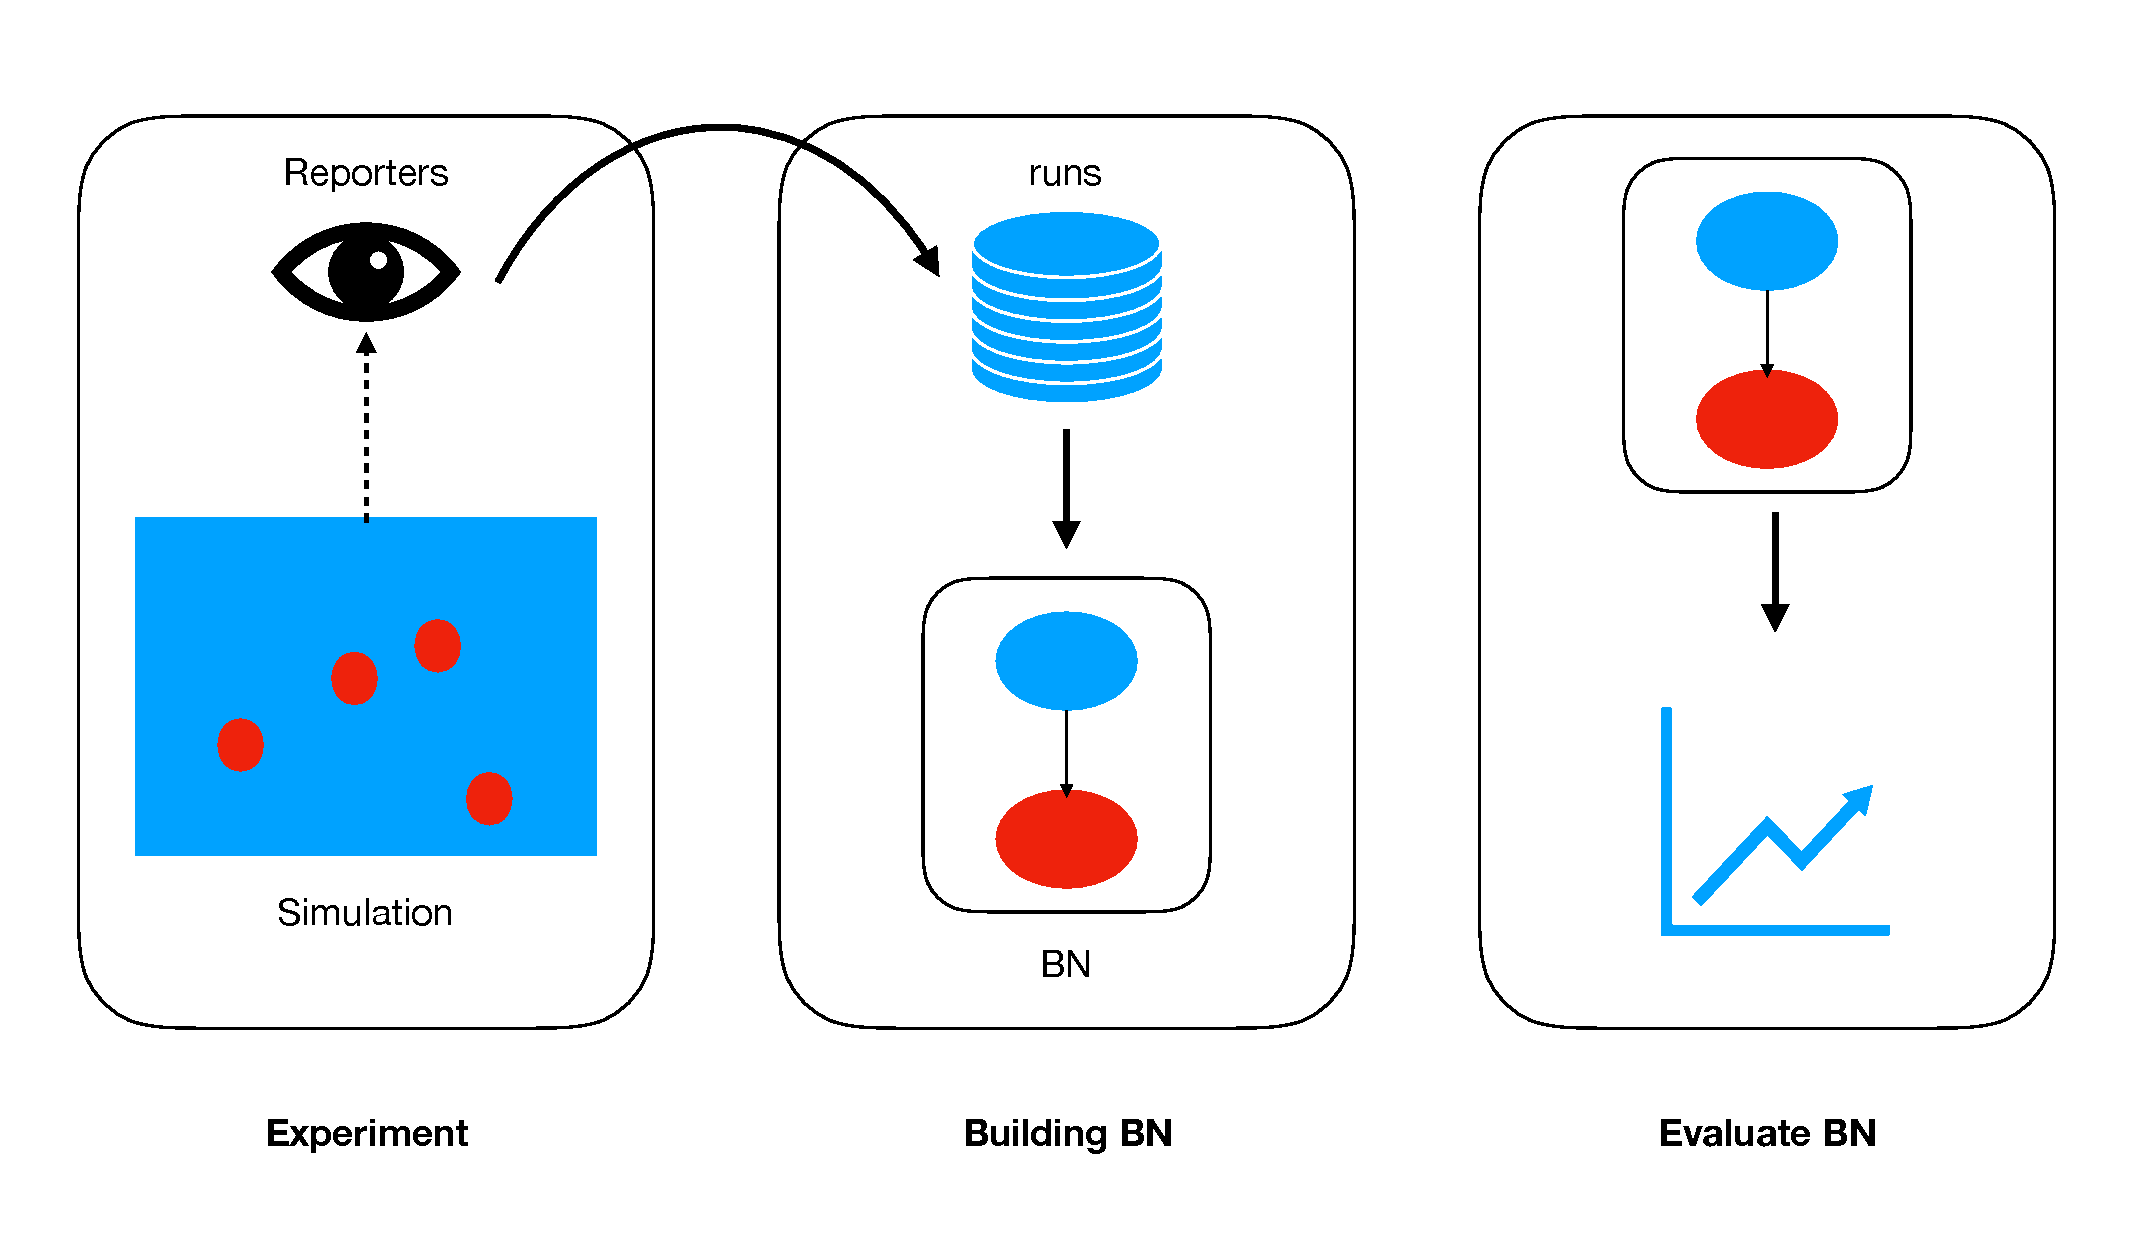
\includegraphics[width=\linewidth]{images/pipeline.pdf}
\label{pipeline}
\caption{Method for evaluating automatically generated Bayesian Networks from simulations.}
\end{figure}


\section{Setting-up an Experiment}
An experiment consists of a simulation and reporters. Reporters are defined separately from the simulation because they are not inherent to it - they are defined with respect to what we want to know about the simulation.

\subsection{Simulation}

\subsubsection{Structure of a simulation}
In the simulation, we are simulating some sort of criminal scenario - a theft, usually. Or we are simulating purely for the theoretical things. The simulation can be as precise as necessary, but there are certain things that need to be present: we need to have states that happen, there needs to be evidence for those states as well. The granularity of the simulation and its complexity depend on the modeller and her requirements.

\subsubsection{Spatial and Non-spatial simulations.}
I'm discussing two types of simulations: spatial simulations and non-spatial simulations. In a spatial simulation, an agent's behaviour is mediated with respect to their environment - eg, agents cannot pass through buildings, or cannot see agents that are far away, or can only steal from another agent when that agent is nearby. In a non-spatial simulations, agents can behave and interact with each other, but this is happening without any environment, hence we are simulating an abstraction. In concrete terms, you can think about a non-spatial simulation as a communication game.

For this project, that means that spatial simulations are more complex and interesting than non-spatial simulations, as there are more possibilities for variety.

The simulations were programmed in MESA, a python package that is made for the creation of Multi-agent systems simulations. We define an environment that the agents can interact with, as well as agents that perform some behaviours. Specifics of simulations and agent behaviour are described in the following chapters.

\subsubsection{Predictability and randomness}
Where does the interest of the simulation come from? In one part, agents sometimes do things because they are commanded to do so by the computer \footnote{rephrase, this is always true lol.}. This means that, at the start, a random number generator might `decide' that some agent has a motive, since the random number generator generated a 1 instead of a 0. On the other hand, some randomness arises from interactions between agents, or between agents and their environments. This is where spatial simulations bring additional value compared to non-spatial simulations.

 In non-spatial simulations, all agent states are essentially brought about by a combination of randomly generated numbers, and reasoning rules. For example, if an agent has a tendency to lie (randomly generated), and it has the opportunity for lying (brought about due to the current non-spatial simulation), then it will lie. Hence a combination of behavioural rules and randomly generated numbers results in a state of `agent lies' of 1.
 
 However, in spatial simulations, interactions and behavioural rules and randomly generated numbers are all brought together: if an agent is near another agent (chance interaction), and it has a tendency to steal (randomly generated), then it will attempt (but might not succeed) in stealing. Here the behavioural rule might lead to a more interesting/complex/complicated outcome than in the non-spatial simulation.
 


\subsection{Reporters (as Random Variables)}

In the simulation, certain states can be brought about. For example, an agent can succeed in stealing an object, or in lying, or in having a motivation (or in not having those things). We need a way to observe these states: this is where reporters come in. A reporter reports the outcome of a relevant event or state in the simulation, and is embedded in the code. If an event happens (or does not happen), the reporter reports that the event is true (or false). In essence, the reporter ($R$) is a random variable (RV) (for a further explanation of Random Variables, see Chapter 8!). In short, a random variable maps an event ($e$) to a truth value:

\[ R : e \rightarrow \{0, 1\} \]

Not all the states in the simulation have a reporter associated with it - otherwise I could build infinitely many reporters. I could have reporters for names, for $agent\_Q\_at\_x\_1\_y\_200$. Hence, I only created reporters for states I deemed relevant for the scenario that I am investigating. Here is a subjectivity gap. I can imagine that in my simulation of the Grote Markt (see later chapter), there is some part of the simulation that by chance geometry, lends itself to an easier job for the thief than another part of the simulation. If the thief and victim spawn near this point, then the probability of the thief succeeding will be higher. Increasing the granularity of the reporters might help us determine if there is a spot like this. However, I did not implement this level of granularity in the simulation (yet), because that is a local and specific part, and does not fit into the more global scenario description (the scenario of theft is spatially-free).

The global state of one run of the simulation, is the combination of all reporters.

\[ G = (e_0 \rightarrow \{0, 1\} \times e_1 \rightarrow \{0, 1\} \times ... \times e_n \rightarrow \{0, 1\})\]
 or,
 
\[ G = R_1 \times R_2 \times... \times R_n\]
for $n$ reporters.

Then, we collect these global states over the number of runs that we do for each experiment, which results finally that the output $O$ of this stage of the method, is a series of global states, one for each run:

\[ O = (G_0, G_1, ... G_{runs})\]


\section{Creating a Bayesian Network from a Simulation Automatically}

The output of an experiment is the collection of runs $O$, where each run is the global state $G$ of the simulation, as measured by the random variables $R$. Semantically, it fits that reporters are random variables, as the reporters become the nodes in the Bayesian Network.

Once we have a collection of states and runs, we can give this to an automated Bayesian Network learner, such as those implemented in pyAgrum. These learners can interpolate a Bayesian Network using algorithms, such as Greedy Hillclimbing and K2. This results in automatic generation of the Bayesian Network which is solely based on the data that is collected in $O$. 

For more detail on these algorithms watch this space.
K2 and temporal restraints.  No restraints on evidence (evidence can connect to each other)


\section{Performance Measures}
To get perspective on the performance of the models, we measure their accuracy and their root mean square error.
We generate a training set of $m$ entries and a test set of $n$ entries, by running the simulation respectively $m$ and $n$ times. At every run, we collect the state of the simulation from the reporters. This results in $m$ rows for the training data and $n$ rows for the testing data. The K2 algorithm is trained on the full $m$ entries of the training set, which results in a Bayesian network. The number of runs $n$ and $m$ depend on the simulation, but $n$ is always 10\% of $m$.

The accuracy is calculated on the testing set. Every row in the testing set has a set number of elements: one element for each reporter. For every row, at random, one element in the row is obscured. The rest of the row is passed as input to the Bayesian Network, we set it as evidence. This means that there is one node that we do not set evidence on, which is the node that represents the obscured reporter. Due to the evidence now set in the network, this node now has a posterior probability. 

For accuracy: We round the posterior probability to either 0 (if posterior $\leq 0.5$) or to 1 (if posterior $>0.5$). The rounded posterior is compared to the obscured element. If they match, the network has correctly predicted the state of a random reporter in the simulation. If they do not match, the network has made an incorrect prediction. The accuracy is calculated as \[\frac{correct}{total}\]

We also calculate the root mean square error as a way to see how close the posterior of the network is to the state of the world. We do not round the posterior probability, and for each row compute \[\sqrt{\frac{\sum_i^N (state_i - posterior_i)^2}{N}}\] 


\section{Evaluating the Bayesian Network}

We want to evaluate different aspects of the Bayesian Network: structural criteria, performance criteria and human criteria.

\subsection{Structural Criteria}
\begin{enumerate}
\item (temp) Hypotheses are ordered temporally. Following the cause-consequence idiom.
\item (con) Evidence connects to hypotheses.
\item (rel) Relevance: All relevant events are in the BN, all irrelevant events are outside of the BN.
%\item (exc) All events that are irrelevant are not included in the scenario BN.
%\item (exh) All events that are relevant are included in the scenario BN.
\item (ind) Independent events are not connected to each other.
\end{enumerate}

\subsection{Performance Criteria}
\begin{enumerate}
\item The accuracy 
\item the Root Mean Squared error
\item The sensitivity analysis of the output node
\item Evidence updates the posterior in the correct direction.


%\item The accuracy of the network is not lower than the inherent randomness of the simulation. Explain how to calculate accuracy and RMS here.
%\item The strong view: probabilities in the network correspond exactly to probabilities in the simulation.
%\item The weak view: Updates on evidence in the network go in the same direction as updates on evidence in the simulation.
%\item Sensitivity analysis shows that no simulation-irrelevant event influences some output \footnote{rephrase}
\end{enumerate}

\subsection{Human Criteria}
\begin{enumerate}

\item How robust is the network against a loss of precision? \citep{Druzdzel2013}.

\item Do we think that a human can find these numbers?
	\begin{enumerate}
	\item How robust is the network against disturbances around the mean (problem with precision)?
	\item How robust is the network around rounding to arbitrary intervals?
	\end{enumerate}
\end{enumerate}

Now that we've established how the automatically generated Bayesian Networks are going to be judged, we can show cautiously in the next chapter how well they are holding up!


				% 75 
%% Activate the following line by filling in the right side. If for example the name of the root file is Main.tex, write
% "...root = Main.tex" if the chapter file is in the same directory, and "...root = ../Main.tex" if the chapter is in a subdirectory.
 
%!TEX root =  mainMastersProject.tex

\chapter[Simple Non-Spatial Simulations]{A Simple Stabbing - Non-Spatial Simulations and their Bayesian Networks}

\section{Introduction}
Here I talk about the credibility game and Charlotte Vlek's Stabbing Bayesian Network example.

In these non-spatial simulations, there are agents, and they interact with each other, but there is no environment for them to interact in. So the simulation is a pure combination of the probabilities assigned to each state transition (or something along those lines). In a sense, the probability for an agent to `stab with knife' purely depends on the probability of `motive' and `opportunity'. Compared to a spatial simulation, where `opportunity' is more complex, as it involves proximity to victim which arises from the simulation and not from some random number generator.

These non-spatial simulations are boring, but they are necessary first steps: after all, if we cannot make BNs out of these predetermined (the probabilities in each run are not predetermined, but the distributions that they are drawn from, and their thresholds, are), then the rest of our endeavours will be fruitless. On the other hand, if the process for creating and evaluating these simple simulations work well, then we can proceed to modelling more complex, spatial simulations.

In this part, I have two experiments. One simple experiment meant to be a replication of Charlotte Vlek's Bayesian Network in xxx \footnote{rephrase}, and another simple experiment mainly meant to test the evaluation criteria for the Bayesian Networks, as outlined in the previous chapter.

\section{Method}
%There are two methods outlined here, one for each initial experiment.

Take the Vlek networks from Vlek Jurix 2015.

The general story is: Jane and Mark had a fight, but Jane had a knife. Mark died. 

Then, there are two specific scenarios that can explain why Mark died. In scenario one, Jane stabbed Mark, and then he died. In scenario 2, Jane threatened Mark with the knife, Mark hit Jane, Jane dropped the knife, Mark fell on the knife, and Mark died by accident. There are two separate networks for these scenarios.

I'm going to create two separate networks, and then also see if I can merge them, by creating a Jane-and-Mark-knife simulation, assigning some random probabilities that correspond to the story, and see what the K2 algorithm makes of it. Then I will also merge the two networks to see if the K2 can deal with mutually exclusive nodes (eg: `Mark died by accident' should rule out `Mark died by stabbing').

So, I created some logical rules, either atoms or rules, and we can process in the simulation these using standard forward chaining inference. Every atom has a prior probability, and every conclusion of a rule has a probability given the F/T state of the premises. At every step, the simulation checks which new sentences are true, applies a rule with a given probability, and counts the outcome.

This does mean that rules at the end are not triggered as often as rules in the beginning, even if they have the same trigger probability (they are on other sides of the chain, more needs to be have happened to conclude that Mark died).

\subsection{Behavioural rules for the simulation}

\begin{table}
\begin{tabular}{|c|c|c|}
 \hline
 Premise & Conclusion & P(conclusion) given premises\\
 \hline
  & Jane and Mark fight   & 20   \\
  & Jane has knife & 70 \\
  \color{blue}Jane and Mark fight, Jane has a knife & Jane stabs Mark with knife & 1 \\
 \color{red}Jane and Mark fight, Jane has a knife & Jane threatens Mark with knife & 3 \\
  \color{red}Jane threatens Mark with knife & Mark hits Jane & 90 \\
  \color{red}Mark hits Jane & Jane drops knife & 50  \\
  \color{red}Jane drops knife & Mark falls on knife & 10 \\
  \color{red} Mark falls on knife & Mark dies by accident & 60  \\
  \color{blue}Jane stabs Mark with knife & Mark dies  & 70 \\ 
  \color{red}Mark dies by accident & Mark dies & 100  \\ 
\hline
\end{tabular}
\caption{For combined scenarios: blue rules belong to scenario 1, red rules belong to scenario 2, and black rules belong to both.}
\end{table}

This was done using forward chaining, with a time index, which means that a rule could only be triggered at one time (otherwise the probabilities get messed up). So we have a forward chaining rule, which means that if the premises of some rule are true, there are no excluding facts true, the timestep is correct, and the random number generator generated a number that is lower than the probability threshold, we find that the conclusion is true, and add it to our found facts. We keep doing this.

Vlek's paper contains no probabilities, so I'm just making some up. The logical sentences are reporters in the simulation, and then I let the simulation run for 10,000 times. 

\section{Results}
We succeeded in generating three different BNs:  One for scenario 1, one for scenario 2, and one for the combined network (Figure~\ref{kb1}, Figure~\ref{kb2}, Figure~\ref{full}).

\begin{figure}[htbp]
\begin{center}
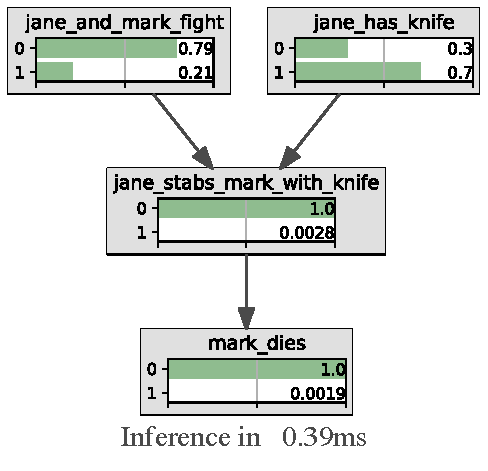
\includegraphics[]{images/Kb1.pdf}
\caption{Automatically generated BN with K2 and the above forward chaining rules, scenario 1.}
\label{kb1}
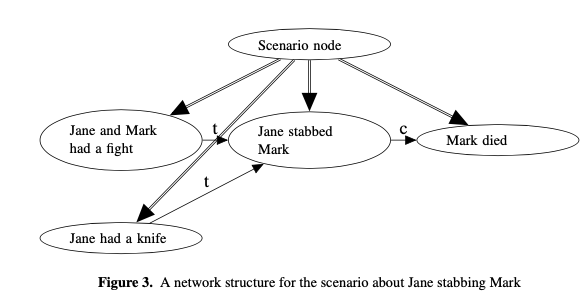
\includegraphics[scale=0.55]{images/vlek2015a.png}
\caption{Vlek BN.}
\label{vlek1}
\end{center}
\end{figure}


\begin{figure}[htbp]
\centering
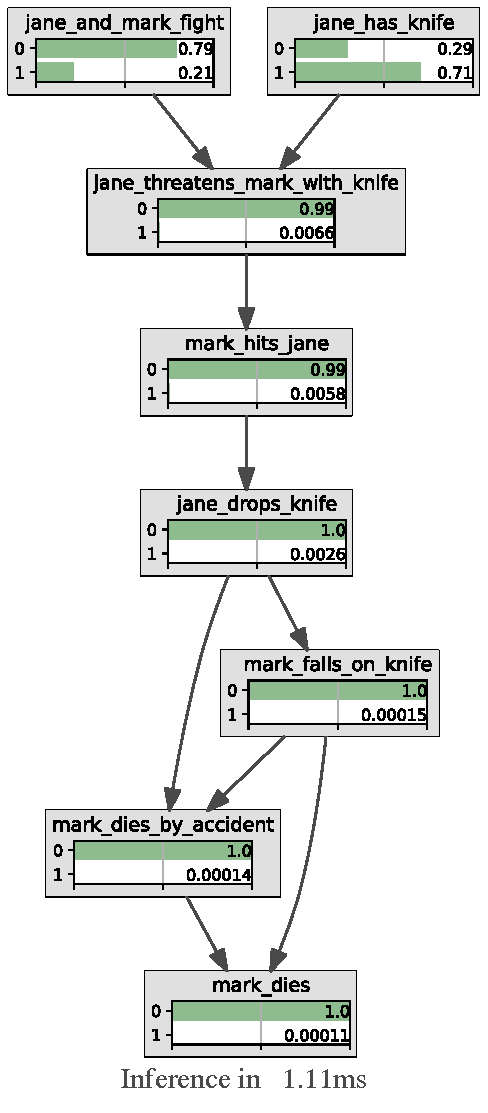
\includegraphics[scale=0.7]{images/Kb2.pdf}
\caption{Automatic generated BN with K2 and above forward chaining rules, scenario 2}
\label{kb2}
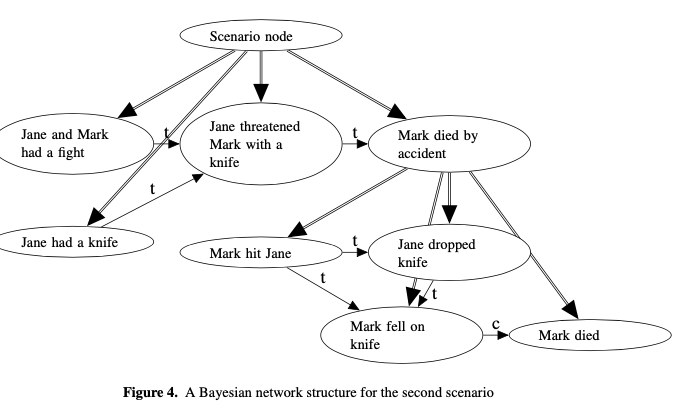
\includegraphics[scale=0.55]{images/vlek2015.png}
\caption{Vlek BN.}
\label{vlek}
\end{figure}


\begin{figure}[htbp]
\begin{center}
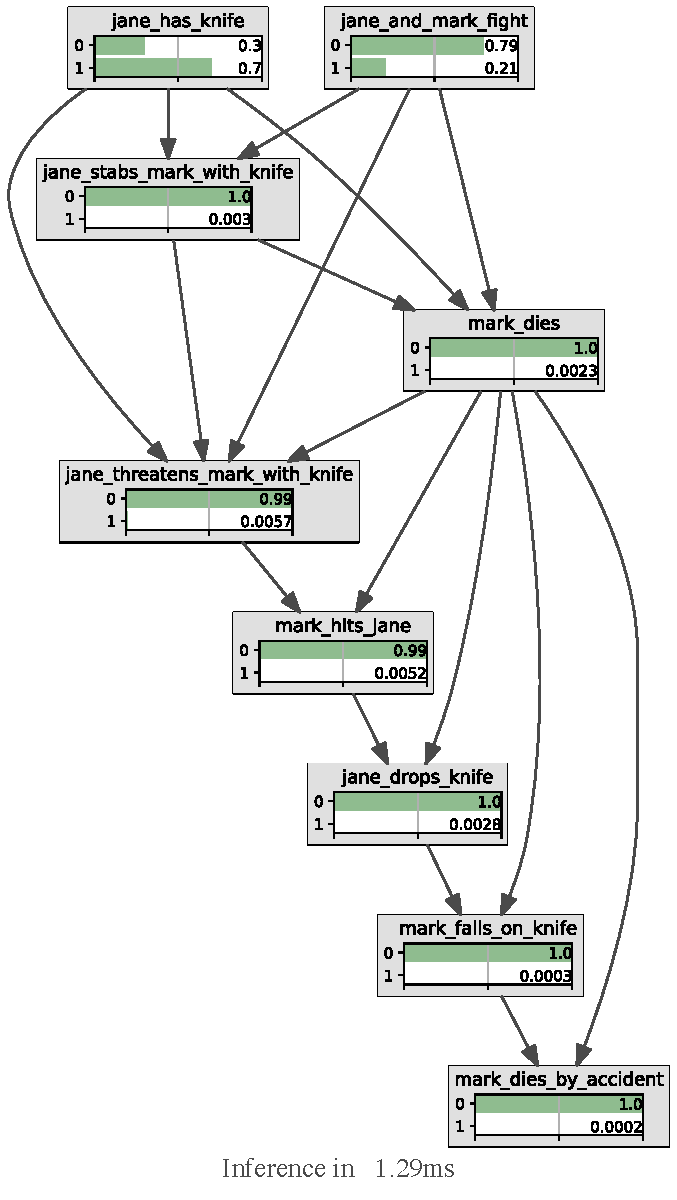
\includegraphics[scale=0.8]{images/Kb.pdf}
\caption{Automatically generated BN with rules from both scenarios included.}
\label{full}
\end{center}
\end{figure}

\section{Discussion}
How well do these networks evaluate compared to the criteria we set out initially, and how well do they compare to the Vlek networks, and the criteria set out in Vlek 2015?




\subsection{Structural Criteria}
\begin{enumerate}
\item (temp) Events are ordered temporally - scenario-like.

In the forward chaining knowledge base, we have premises and conclusions. If we take the event in a conclusion, then we know that the premise of that rule, is the parent of that node in the Bayesian Network. (again, rephrase this is so vague. Maybe make it a rule or smth). The two ``premiseless'' events Jane and Mark fight, and Jane has a knife, are also parentless in the simulation. In this sense, the structure of the Bayesian Network reflects the structure of the inference rules that we set out.

We see that in both the separate networks, the temporal ordering of the nodes is correct - every node has as a parent a node that represents an event that would have happened beforehand. In the combined network, this is not the case: mostly the temporal links are represented ok (eg: the chain of events from "Jane threatening Mark" to "Mark dies by accident" is represented correctly), however, this chain of nodes all has as a parent "Mark dies", which would, temporally, occur only after "Mark falls on knife" occurs. This means that in the combined Bayesian Network, we cannot satisfy the temporal ordering constraint due to the conditional probabilities between the events (eg: if Jane stabs Mark, then she cannot threaten him after, which is a relation that `inhibits' the `Jane threatening Mark' node - eg: there is a conditional relation between the two nodes, but not a temporal or causal one). As a conclusion about this criteria: Maybe temporal ordering should just hold within scenarios and not between scenarios, because we get into these sorts of causal messes. Or we should use the scenario node to organise different scenarios together. Idea: scenario node could cause temporal ordering, but what in cases with much shared evidence?

\item (con) Evidence connects to hypotheses.

In the original network, we have no evidence, so it is not included into this one. However, I might add some evidence to test the Performance Criteria.

\item (exc) All events that are irrelevant are not included in the scenario BN.

This criteria, and the next one, are freebies, because we are just copying a network that already exist - our set of relevant events is the same as that in the original network by Vlek. We do not have any irrelevant event because we can see that all events are connected to each other, and all events reflect an underlying `decision' by an agent.

\item (exh) All events that are relevant are included in the scenario BN.

We have included all relevant events - all the events in the knowledge base are also in the network.

\item (ind) Independent events are not connected to each other.

This is not entirely correct in the uncombined networks (and also not correct in the combined network) - If Mark dies by accident, this is only dependent on Mark falling on the knife, and not also on Jane dropping the knife (since all cases where Mark dies by accident are also cases where Mark falls on the knife, we don't need a separate condition for Jane dropping the knife). This is probably due to an insufficient number of runs (eg: the probability that this happens is very low and we might not have enough data to correctly estimate it).


\end{enumerate}

\subsection{Performance Criteria}


\begin{enumerate}
\item The accuracy of the network is not lower than the inherent randomness of the simulation.



\begin{figure}[htbp]
\begin{center}
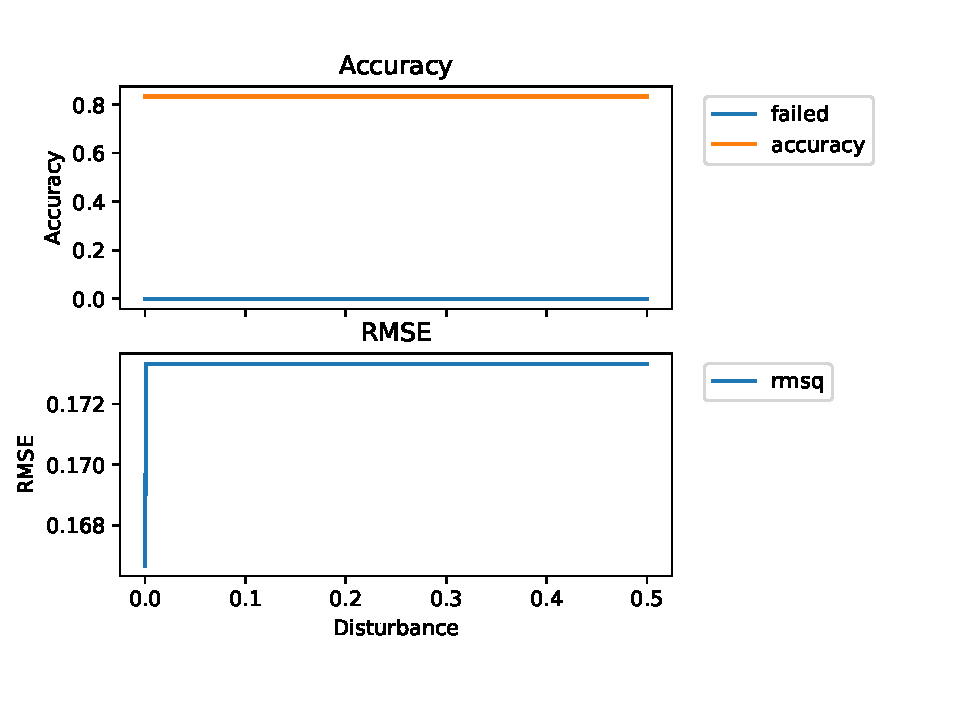
\includegraphics[]{../experiments/VlekNetwork/plots/performance_KB1.pdf}
\caption{Accuracy (100\% to 0\%) and Root Mean Square error (1 - 0) for rounding to different intervals in network 1.}
\label{kb1a}
\end{center}
\end{figure}

\begin{figure}[htbp]
\begin{center}
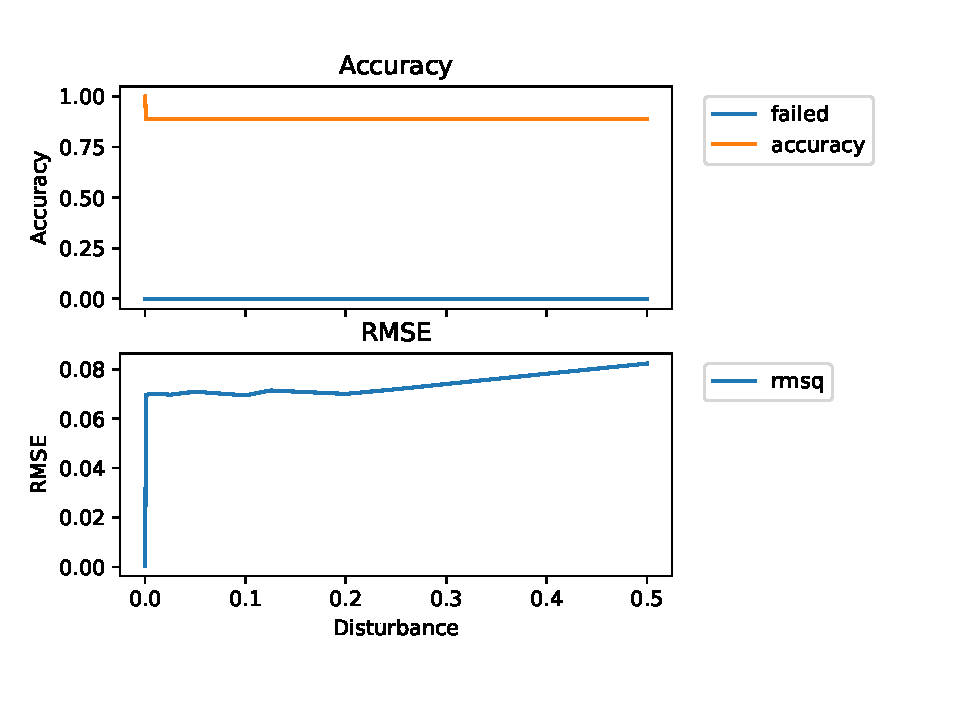
\includegraphics[]{../experiments/VlekNetwork/plots/performance_KB2.pdf}
\caption{Accuracy (100\% to 0\%) and Root Mean Square error (1 - 0) for rounding to different intervals in network 2.}
\label{kb2a}
\end{center}
\end{figure}

\begin{figure}[htbp]
\begin{center}
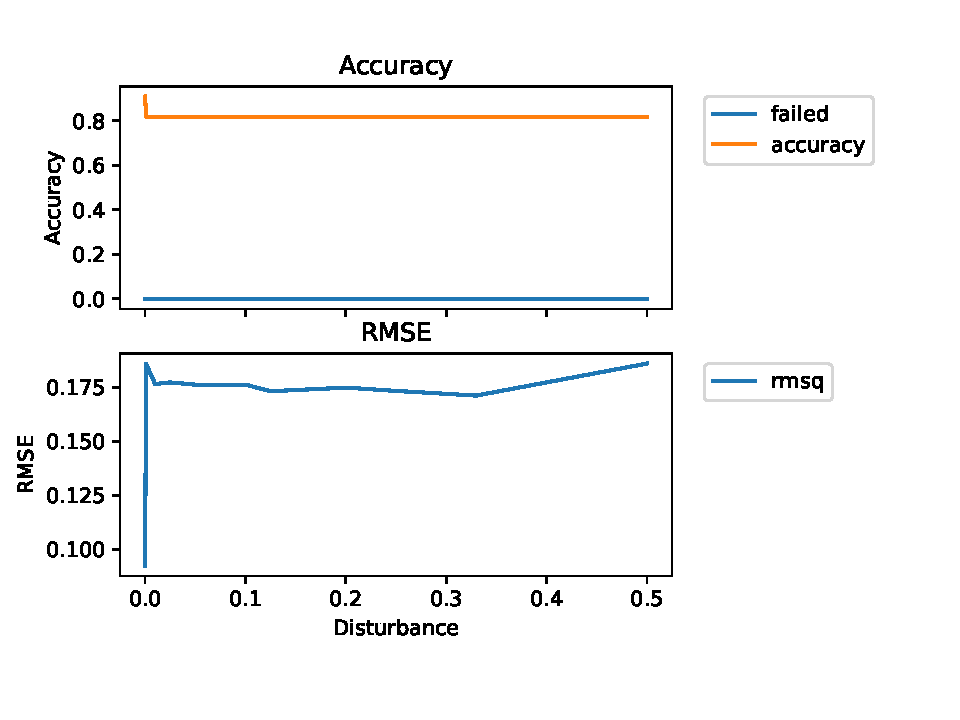
\includegraphics[]{../experiments/VlekNetwork/plots/performance_KBFull.pdf}
\caption{Accuracy (100\% to 0\%) and Root Mean Square error (1 - 0) for rounding to different intervals in the full network.}
\label{fulla}
\end{center}
\end{figure}

We see that as the disturbance increases (eg we round to larger intervals), accuracy obviously decreases, and RMS increases. But these decreases and increases are not that drastic, and overall performance is still pretty good (eg even for the worst, accuracy is still near 0.88)

\item The strong and the weak view.

The strong view: probabilities in the network correspond exactly to probabilities in the simulation. The weak view: Updates on evidence in the network go in the same direction as updates on evidence in the simulation.

\begin{table}
\begin{tabular}{|c|c|c|}
 \hline
 Conclusion &P(conclusion) given premises & P(event) given premises\\
 \hline
 Jane and Mark fight   & 20 &  20.87   \\
 Jane has knife & 70 & 70.23 \\
 Jane stabs Mark with knife & 1 & 2.05 \\
 Mark dies & 70 & 75.46 \\ 
\hline
\end{tabular}
\caption{For only scenario 1.}

\begin{tabular}{|c|c|c|}
 \hline
 Conclusion &P(conclusion) given premises & P(event) given premises\\
 \hline
 Jane and Mark fight   & 20 &  20.87   \\
 Jane has knife & 70 & 70.23 \\
 Jane threatens Mark with knife & 3 & 3.88 \\
 Mark hits Jane & 90 & 90.21 \\
 Jane drops knife & 50 & 50.09 \\
 Mark falls on knife & 10 & 11.13\\
 Mark dies by accident & 60 & 61.25 \\
 Mark dies & 100 & 99.79 \\ 
\hline
\end{tabular}
\caption{For only scenario 2}
\end{table}

For both scenarios, the probabilities in the network are very similar to the probabilities in the ground truth (simulation). There is a
loss of precision, which is the worst in case of `Mark dies' in the first scenario, which is estimated at 75\% by the network, but in fact in the simulation is only 70\% probable. I don't know where this comes from. Apart from that, all divergences for the original probabilities are within 2\%. This means the strong view does not hold, but the weak view does (updating on evidence gets us with probabilities that are closer to the simulation probabilities than before).


\begin{table}
\begin{tabular}{|c|c|c|}
 \hline
 Conclusion &P(conclusion) given premises & P(event) given premises\\
 \hline
 Jane and Mark fight   & 20 &  20.87   \\
 Jane has knife & 70 & 70.17 \\
 Jane stabs Mark with knife & 1 & 2.06 \\
 Jane threatens Mark with knife & 3 & 3.88 \\
 Mark hits Jane & 90 & 91.50 \\
 Jane drops knife & 50 & 52.97 \\
 Mark falls on knife & 10 & 10.92\\
 Mark dies by accident & 60 & 66.33 \\
 Mark dies (premise: Jane stabs Mark) & 70 & 68.68 \\ 
  Mark dies (premise: Mark dies by accident)& 100 & 98.77 \\ 
\hline
\end{tabular}
\caption{For combined scenarios}
\end{table}

The probabilities of the conclusions in the combined network given the premises, also look relatively similar on a human scale - I assume that a human probability elicitor would not be able to distinguish between a probability of 11.13, 10.92 or 10.00 for the conclusion ``Mark falls on knife". On the other hand, if we round all the probabilities in the network to 10, a human probability elicitor might be able to say that the probability of `Mark falls on knife'' is 0.1 (or 10\%), to exactly that level of precision (so not 0.10, or 0.100). The resulting probabilities might be elicitable, while still meaningfully reflecting the ground truth.


\item Sensitivity analysis shows that no simulation-irrelevant event influences some output \footnote{rephrase}
\end{enumerate}

\subsection{Human Criteria}
\begin{enumerate}
\item Do we think that a human can find these numbers?

The conditional probability tables as displayed in these networks are not great.

	\begin{enumerate}
	\item How robust is the network against disturbances around the mean (problem with precision)?
	\item How robust is the network around rounding to arbitrary intervals?
	\end{enumerate}
	
\item Can a human find this network \& reason with it? All the evidence points in the correct direction, in the weak and strong views we're ok, even for relatively large intervals - we see a sharp drop in accuracy and increase in RMS error at around intervals of 0.33. This would mean, that for these networks, the elicitor should only need to specify probabilities that are 0, 0.33, 0.66, and 1 (eg, round every probability that is not one of these, to one of these). Note, that this is likely different dependent on the complexity of the networks (in some way, lol). This sounds definitely plausible as a lower level. If someone has strong opinions on the CPT then we can always increase precision in certain nodes. Hence, this seems pretty great.


\end{enumerate}




\subsection{Comparison to Vlek 2015}
If we only look at the ordering of the Bayesian Network, we can see that for Figure~\ref{kb1}, the sub-scenario structure is the same as in Vlek 2015 Figure~3, our Figure~\ref{vlek1}. There's no scenario node constraining the network, all the information is contained in the network, no scenario node needed (todo: make the nodes the exact same names).

However, there are differences between Vlek 2015 Figure~4, and the automatically generated BN here. Figure~4 in Vlek 2015 is replicated below in Figure~\ref{vlek} (todo: ask permission?? or just remove). The automatically generated BN is very linear and can be interpreted in a purely temporal way: mark hits jane, jane drops the knife, and due to jane dropping the knife, and mark falling on it, mark dies by accident - and if mark dies by accident, mark dies. The probabilities for all these events (from jane dropping the knife on), are ridiculously low, and don't really make sense (should interpret the small probabilities as e, and not as actual numbers I guess, due to underflow?). 

In Vlek's paper, we see a subscenario: we have the subscenario ``Mark died by accident", which contains events such like mark hit jane, which leads to jane dropping the knife, and mark falling on the knife, and then dying. The coparents of Mark died are the same in this network as in the automatically generated BN, however, we once-again miss the scenario-like construction where mark hitting jane, jane dropping the knife, and mark falling on the knife are connected as part of a subscenario, rather than their ``own" nodes.


Why to choose for subscenarios when it is not required? Tomorrow I will look up why the scenario construction was used and I will see if it does something that I miss? Coherence? But that also travels up the chain? But something with d-separation probably. I'll read the Vlek 2015 again i guess.



In the full final network, we see that the two mutually exclusive scenarios (stabbing vs falling on knife) are excluding each other even without the use of a scenario node - so we can make networks that combine two different stories. This is nice.

\subsection{Quality of scenario}
\begin{itemize}
\item Completeness - have all the parts and not one more. Not a big deal for this simulation, as I've taken all the nodes from Vlek 2015, there's no discussion about granularity.

\item Consistent - no internal contradictions. There is no explicit structure in the final BN that ensures consistency. The probabilities inside the BN need to ensure that. For instance, the only thing that is contradictory in the KB is that jane threatening and jane stabbing, cannot both happen. In the final network (Figure~\ref{full}), there are nodes for both threatening and stabbing. However, the relations of these nodes are such, that when one node becomes more likely (eg, we set evidence on it),  the other node becomes less likely (as we can see in the figure below:

figure here of $\Delta$ P stabbing for increasing values of P threatening. If we know threatening is true, stabbing goes to 0, and vice-versa - and all the consequences of the threatening scenario also go to 0, so it just works. This means that several different scenarios can be combined into one network, and still be mutually exclusive. Both scenarios share some events (as some scenarios can do in real life), but the different scenarios themselves are not separated from each other by structure or construction (as is the case in Vlek~2015).

Do we need the constraint node? Or do we only use that if we have knowledge but no data? what. 11 in Vlek.

We can just straight-up draw a line between two events in order for them to become mutually exclusive, like we do with Jane stabs mark and jane threatens mark. Fenton et al advice against that - we draw a relation between two causes to ensure mutual exclusivity. Fenton doesn't like this even though it satisfies the axioms because 1) the parent cause becomes part of the causal pathway leading to the child cause, which means that you have to involve many more numbers (``meaningless columns''). Fortunately, this is not a problem in the automatically generated BNs, because the algorithm fixes this for us :). Not sure if an extra node is good for the computational complexity of BNs either. Uh. Anyway, even if this is not the case, there are lots of unnecessary numbers in Bayesian Networks anyway (show image here), because there's many combinations of events that just do not happen (eg: mark dies but jane doesn't have a knife, never happens, but is in the table anyway. Unnecessary complexity? Probably a rounding error!!). Anyway, that's a thing. So it doesn't really matter.

Uh. The second objection is that you have to arbitrarily decide which cause is the parent - which doesn't make sense if you interpret the networks causally. Fortunately. there's no causality in this part, its just frequencies so it doesn't matter, we can just pick one and it's fine. So turns out we don't need the constraint node anyway :D

\item Plausible - scenario should correspond to the modellers knowledge about the world. Support can help implausible scenarios to become plausible.


\end{itemize}




\section{Important take-aways}
In this section, I summarise some important take-aways, that will be necessary for the rest of this project. Things that we learn here, will be useful in evaluating the rest.

\subsection{Simulations work}
Even this very simple `forward chaining' simulation (eg: forward chaining with some probabilities attached), can be used to construct meaningful Bayesian Networks. The Bayesian Networks have generally ok accuracy and RMS error, and reflect the structure of the simulation (dependent on the number of runs, that's true). Even when we disturb the CPTs in the table, we get relatively ok accuracy and RMS until  


\subsection{We don't need the scenario node for mutual exclusivity}
Both of Fenton's objections for the direct node connection are not problems for us (yet) - the first one, specifying too many numbers, might become problematic in the future, and the second, about the interpretation of the arcs between nodes is not a problem, because we interpret these links as solely conditional, and not causal. Background information about causal relations between events might help us to order the network, so that it can become more efficient, but this should not affect the ``reasoning'' aspect - eg, even if the structure of the network is different, updating on evidence should produce the same results as before.


\subsection{Resolution and number of runs}
The accuracy of the Bayesian Network improves as the number of runs improves. This is an obvious fact. It has implications for the rest of the network. For example, if we run the network too few times (let's say 10 times), then the network will not be able to estimate the probability of certain states - eg: the probability that Mark hits Jane can be calculated as: $0.7 \cdot 0.2 \cdot 0.03 \cdot 0.9 = 0.00379$, which means that there's a 0.378\% chance that it happens, eg, if we run the simulation a 1000 times, Mark will hit Jane in 4 of them (or, actually, the sentence ``Mark hits Jane" is true in 4 of them). If we go all the way down the chain of unreasonable facts to ``Mark dies accidentally", we get a probability of 0.0001134, which is 1 every 10.000 runs. If we run the simulation 10.000 times, that means that we cannot estimate probabilities that are smaller than 0.0001 - either they occur `accidentally', eg, by chance, and the network estimates that they happen once every 10.000 runs, or they don't happen within 10.000 runs, and the network estimates that these events never happen at all - when in fact, they might happen, but just once every 20.000 runs.

What are the practical implications of this? On this side, that we need enough data to get an accurate prediction. But, if we're thinking about elicitation, this means that if you decide to add an event to a scenario, or a node to a network, you really have to think about the probability that you assign it - a probability of 1 in 10.000 would really mean that this event would only happen once every 10.000 situations (that you are considering - the reference class is never far away). 


\section{Conclusion }

With this part, I have shown that the pipeline works. We can make a simulation using forward chaining, that generates world-states, and those world states can be translated into Bayesian Networks by means of the K2 algorithm, with reasonable accuracy even under rounding. The K2 manages to replicate constraints and merge two different possible scenarios together. So if the real world worked like a simple forward chaining inference method where we knew exactly when a proposition was true (which is, if the state is true, we set the proposition to true in every epoch), then BNs would work flawlessly even if we weren't very great at estimating the correct frequencies precisely.

Sad that the real world doesn't work that way.


%> Dit is de focus van mijn onderzoek!!!

%> ik laat zien welke dingen je allemaal nodig hebt om statistische shit te gebruiken
%> als een van deze dingen niet aanwezig is, is het dus niet mogelijk om BNs te gebruiken in het echt
%> in de simulaties weet je precies welke wetmatigeheden je hebt (want die definieer je met je simulatie/forward chaining etc)
% s> maar die kunnen we dus nooit in het echt vinden. En dus kunnen we BNs nooit in het echt toepassen. end.


				% 0
%% Activate the following line by filling in the right side. If for example the name of the root file is Main.tex, write
% "...root = Main.tex" if the chapter file is in the same directory, and "...root = ../Main.tex" if the chapter is in a subdirectory.
 
%!TEX root =  mainMastersProject.tex

\chapter[Simple Spatial Simulations]{A Simple Robbery - Spatial Simulations and their Bayesian Networks}

Three experiments: 1) getting the bayesian networks with disturbances (). 2) testing the effect of a simulation parameter change on the BN (how different does it become. 3) investigating the effect of hidden information/private knowledge on the network.
Summary:

 The problem is that in the previous chapter, we have established that we have a method to convert a simple, forward chaining simulation, to a collection of data, which then in turn can be used to create a Bayesian Network, that represents the situation in the simulation relatively well (some problems none-withstanding, accuracy and RMS error are generally ok even in increments that people might plausibly be able to estimate ~ intervals of 0.33/0.25-ish). However, this was totally 100\% determined by deterministic forward chaining rules. The real world does not run on deterministic forward chaining rules (as far as we know). At least, we are spatially situated, which means that there are probabilities that will arise out of interactions between agents and their environment. These probabilities are not `set' in the same ways as the probabilities are set in the previous chapter, they arise organically from interactions: eg: an agent has to be located at a door to break in, an agent can be seen by a camera only in some locations of the simulation. We do not know these probabilities a-priori (although we can probably calculate them, I don't know).
 
New idea: We create spatially situated simulations that are more complex, and see if they work the same way/are as accurate \& rms as the previous. Then we will also use these simple spatial simulations to test two hypotheses about 1) the effect of private knowledge and 2) the effect of parameters.


\section{Experiment 1: Generating BNs with disturbances}

In this first experiment, I will be creating an agent simulation of a very simple crime case. I will run the simulation for some number of times, and then automatically generate BNs, based on the K2 algorithm. Then I will change the values of the cpts in the BNs, to see if we can accurately predict the outcome even with low precision in cpts, given the structure of the BN.

\subsection{Introduction}

The scenario that the agents play out goes as follows. There are two agents. They are neighbors. One day, the agent who lives in the house on the right ($R$), walks past the house of the other agent ($L$). $R$ looks inside, if it can. Sometimes it cannot look inside, because $L$ has drawn the curtains. However, if $R$ can look inside, it might see a goodie in the house. It also might not see a goodie, if $L$ has lost the goodie - in that case, the goodie has been lost. However, if the goodie is there, $R$ will know that the goodie is there. Then, because $R$ is a rational agent, it will try to calculate the worth of the object, and if it might want to steal it. It can decide to target the object. If $R$ knows and targets the object, $R$ has a motive. Then, $R$ attempts to break into the house by breaking the lock on the door, grabbing the goodie, and running away to its own house.  Meanwhile, $L$ is returning home. If $R$ thinks that $L$ might have seen it stealing, $R$ will flee home, with or without the goodie. $L$ has also hung up security cameras on the outside corner of its house, that might serve as evidence against $R$.

With regards to the end, there can be three outcomes: either the goodie is lost, the goodie is not lost but was stolen successfully, or the goodie is not lost and wasn't stolen successfully ({\color{red}does this mean that there was always a stealing attempt? check in jup}). The environment of the agents is very simple, just two `houses' (rectangles, really). The environment and the agents (with their vision parameter) are shown in Figure~\ref{env}.

\begin{figure}[htbp]
\begin{subfigure}{.5\textwidth}
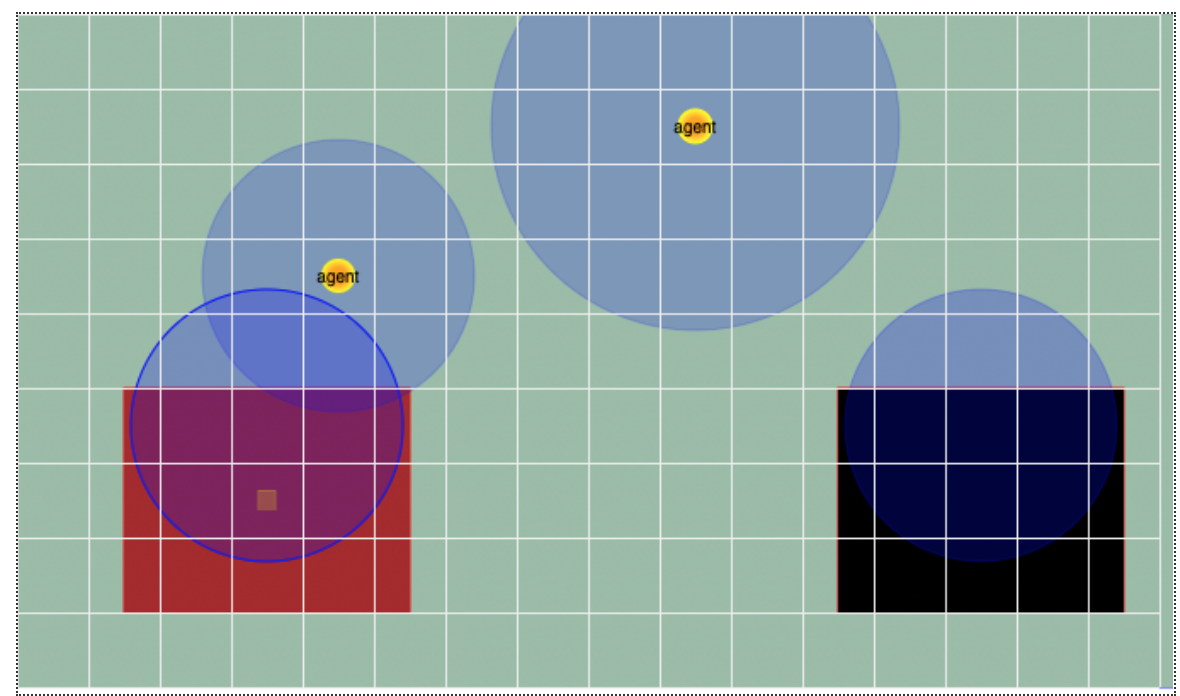
\includegraphics[width=\linewidth]{images/sim1.png}
\caption{The simulation with the 2 agents.}
\end{subfigure}
\begin{subfigure}{.5\textwidth}
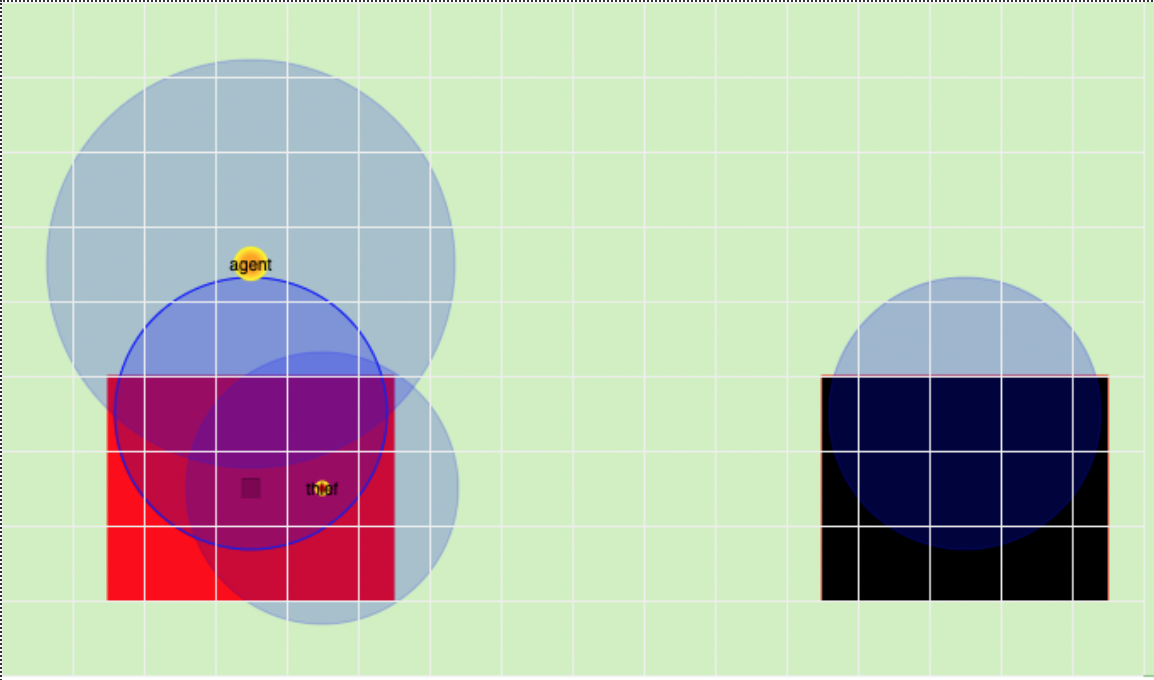
\includegraphics[width=\linewidth]{images/stealing.png}
\caption{The agent attempts to steal something but flees when it thinks that it is noticed.}
\end{subfigure}
\caption{Agents behaving badly in simulation.}
\label{env}
\end{figure}

\subsection{Methods}
There are four things to be explained here: the agent behaviour, the operationalisation of the random variables, the simulation (meta-)parameters, and the process through which the cpts of the given BN is to be disturbed.

\subsubsection{Agent behaviour}
flowchart here.

\subsubsection{Operationalisation of the RVs}

The operationalisation of the random variables is very important. In the table below are all the reporters and how they are defined.

\begin{adjustbox}{center}
\footnotesize
\centering
\begin{tabular}{|l|l|}
 \hline
 RV &Operationalization\\
 \hline
lost\_object   & A random number generator (0, 1) generates a number. If the number $\leq 0.2$, the object is lost.\\
curtains & A random number generator (0, 1) generates a number. If the number $\leq 0.8$, the house has no curtains.  \\
raining & A random number generator (0, 1) generates a number. If the number $\leq 0.5$, it is raining.   \\
know\_object & if we see an object in our vision that is not our own, and we are not already targeting some`
thing else  \\
target\_object & if we know the object exists, and we consider the value of the object higher than our risk threshold.  \\
motive & if we have a target \\
compromise\_house & if we are adjacent to the target's house's door, and we have a breaking and entering skill of greater than 5. \\
flees\_startled & if we see another agent and we haven't been observed yet  \\
successful\_stolen & if we're not in someone's house anymore and we have the object in our possession \\ 
E\_s\_spotted\_by\_house&  {\color{red} todo fill in}. \\ 
E\_disturbed\_house&   \\ 
E\_object\_is\_gone&   \\ 
E\_broken\_lock&   \\ 
E\_s\_spotted\_with\_goodie&   \\ 
E\_private&   \\ 
\hline
\end{tabular}
\end{adjustbox}

\subsubsection{Simulation parameters}
Number of runs: 1000

\subsubsection{Disturbing the cpts}
We generated only one Bayesian Network, with the data we collected from the simulation. Then, we create many new networks, with this network as a basis. We do not change the number of nodes (we do not leave out or add nodes), nor the structure of the Bayesian network. We only change the values in each node's conditional probability table (cpt). In this case, we round the values in the cpt's, such that the BN becomes increasingly less precise. The intuition behind this is, that when expert users are going to elicit the probabilities, we do not know how robust the network is against smaller and larger imprecisions in the elicited probabilities. By simulating such imprecisions, we can compare the accuracy and rmsq error of the more imprecise networks to the ground truth of the `real' network. 

We round every value in the cpts $c$ to each of $i, i \in \{\text{no disturbance}, 0.05, 0.1, 0.125, 0.2, 0.25, 0.33, 0.5\}$, according to \[ floor(\frac{c}{i} + 0.5) \cdot i.\]



\subsection{Results}

See Figure~\ref{laptop}


\begin{figure}[h]
\begin{center}
\begin{subfigure}{.7\textwidth}
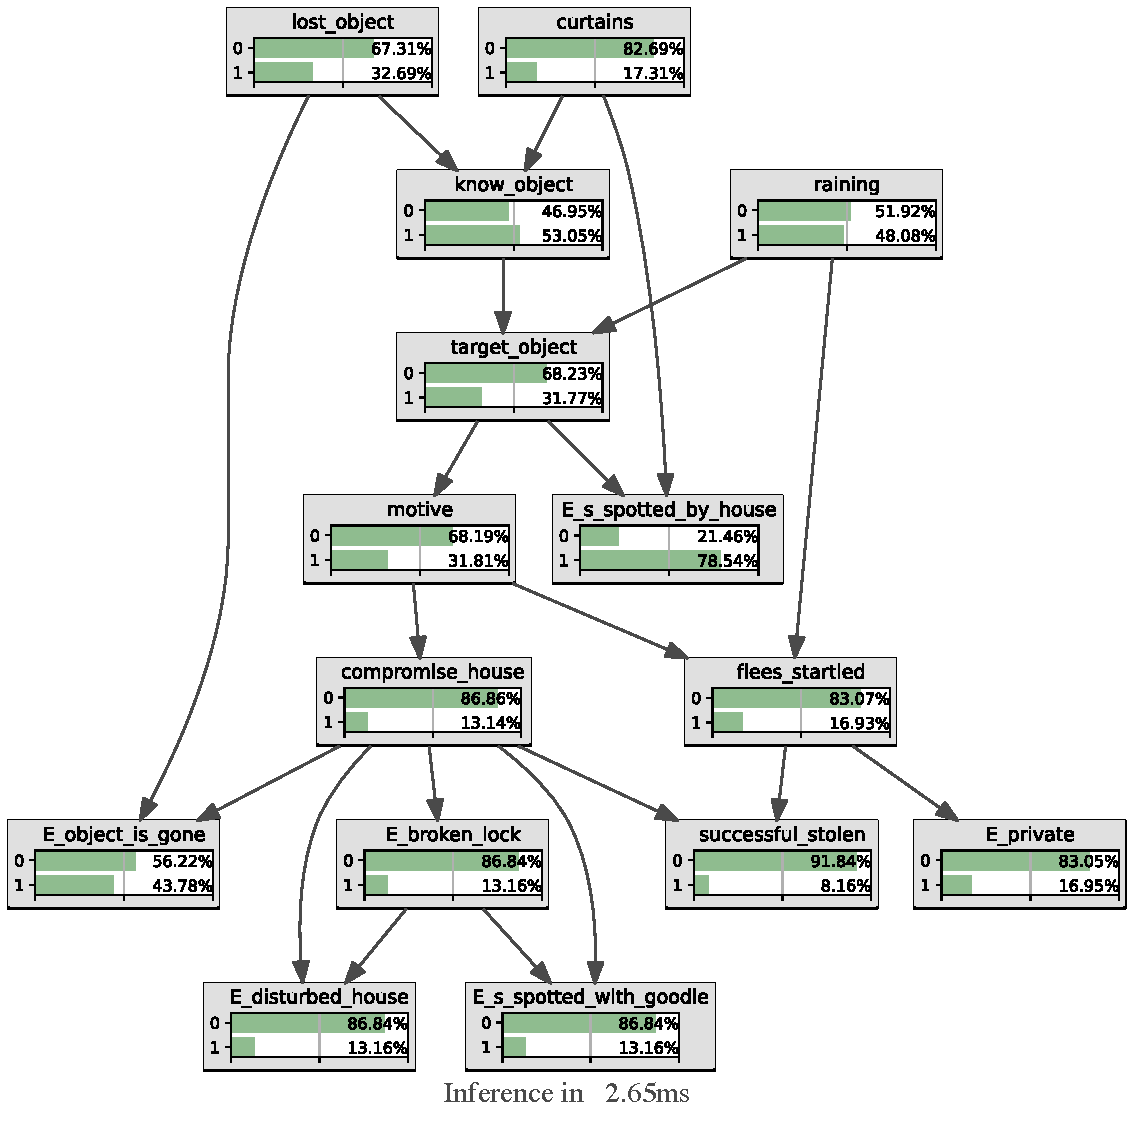
\includegraphics[width=\linewidth]{../experiments/StolenLaptop/bnImage/BNIMAGEStolenLaptop.pdf}
\caption{network structure}
\label{laptopAcc}
\end{subfigure}
\end{center}

\begin{subfigure}{.5\textwidth}

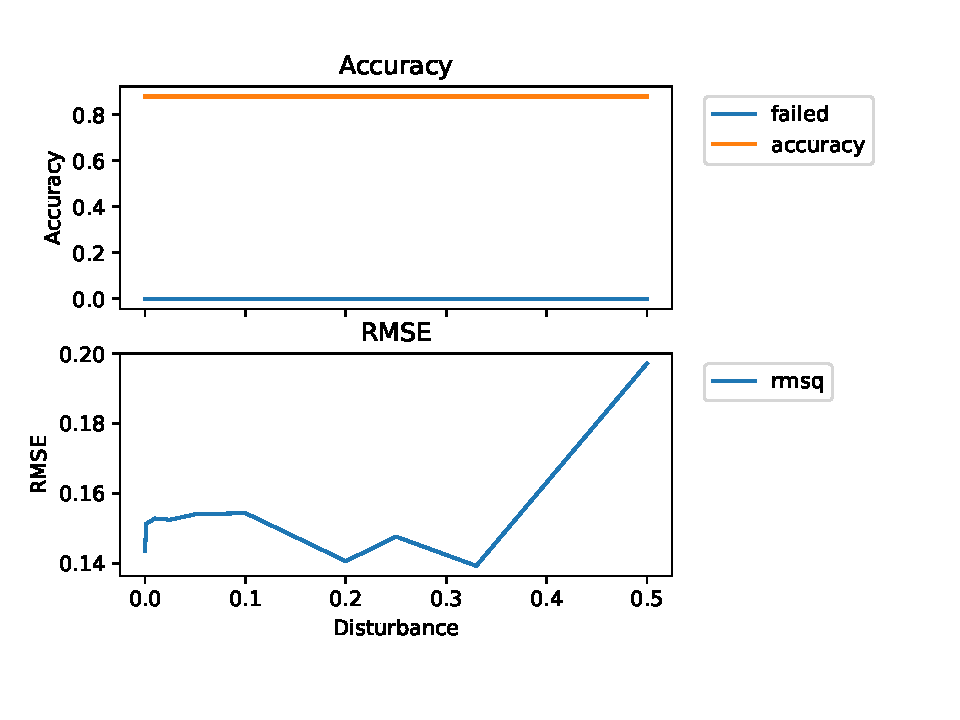
\includegraphics[width=\linewidth]{../experiments/StolenLaptop/plots/performance_StolenLaptop.pdf}
\caption{Accuracy (100\% to 0\%) and Root Mean Square error (1 - 0) }
\label{laptopAcc}
\end{subfigure}
\begin{subfigure}{.5\textwidth}

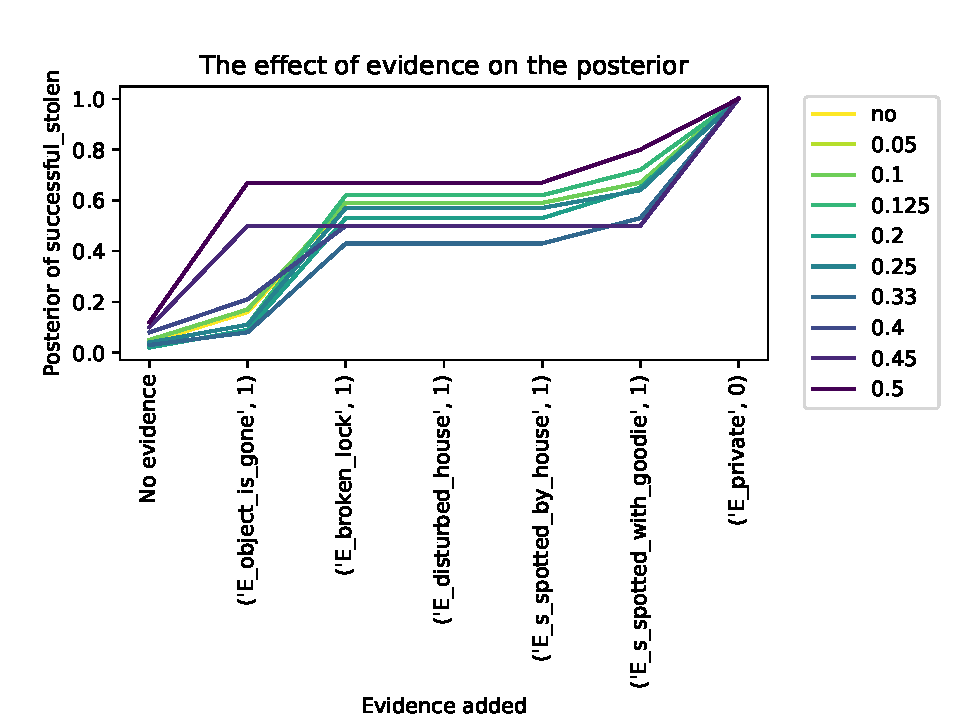
\includegraphics[width=\linewidth]{../experiments/StolenLaptop/plots/posterior_StolenLaptop.pdf}
\caption{effect of evidence on posterior}
\label{laptopPosterior}

\end{subfigure}
\caption{The network, the accuracy and root mean square for rounding the cpts to intervals, and the effect of evidence on the posterior for stolen laptop simulation.}
\label{laptop}
\end{figure}


%\begin{figure}[h!]
%\begin{center}
%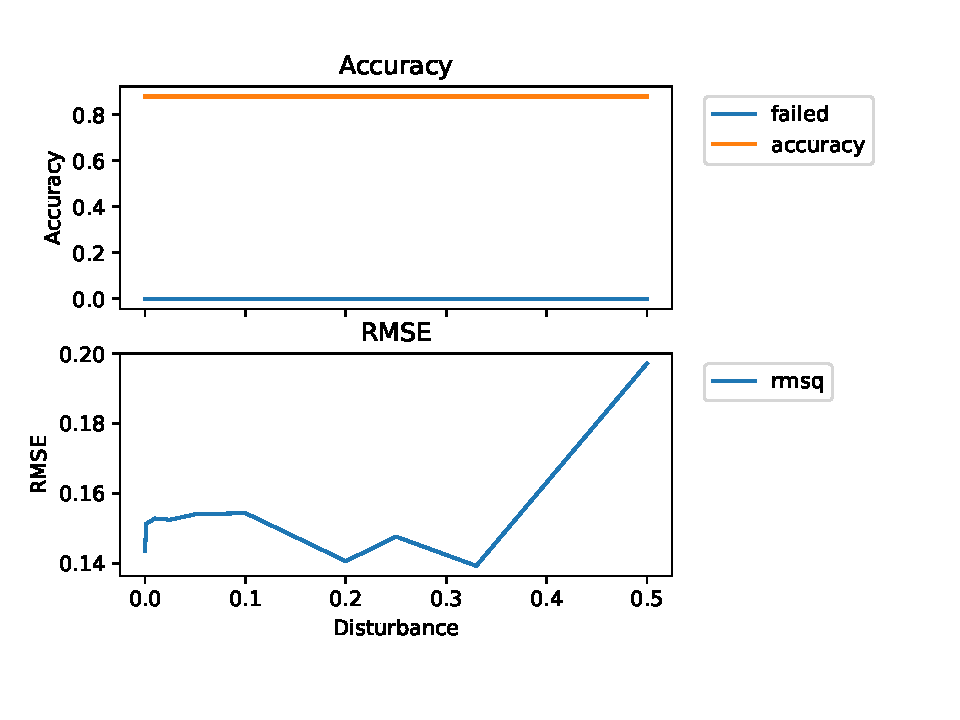
\includegraphics[]{../experiments/StolenLaptop/plots/performance_StolenLaptop.pdf}
%\caption{Accuracy (100\% to 0\%) and Root Mean Square error (1 - 0) for rounding to different intervals in stolenLaptop network and simulation}
%\label{laptopAcc}
%\end{center}
%\end{figure}



Overall pretty accurate. This shows that small disturbances in rounding - and even larger disturbances in rounding, such as to 0.25 or even 0.33, does not matter very much for the accuracy of this specific network. 

{\color{red} todo: add automatic table with accuracies and rms generated}.


\subsection{Discussion}

The network itself makes sense. The spurious node `raining' is not connected to any other node, because the rain should not affect what happens.

The fact that these networks can be rounded without losing accuracy, means that even with a lack of precision in the ctps of the network, the network is still able to accurately predict outputs - eg, whether a node is going to be true or false given a set of evidence. Changing the precision of the network does not change the network structure itself, this is kept constant - it is generated first, and then the cpts are rounded to arbitrary intervals. 

This shows that even when this network's cpt's only contain probability values, [0, 0.33, 0.66, 0.99], we still get the reflection of the evidence in the network. 

\subsubsection{Network structure}

Problem: the disturbance of the cpts means that we're only disturbing the cpts, and not the structure of the network itself. If we look at the ordering of the non-evidence nodes in the network, then we can see that they are ordered temporally - parent nodes happen before child nodes. However, there are many sibling-nodes (nodes with the same parents), and how these nodes relate to each other temporally cannot be understood from the BN alone (does compromise house come before or after flees startled?). 

Knowing to which parent node some pieces of evidence should connect is also not straightforward: evidence could connect to more or fewer parent nodes than they are now. Due to the limitations of the K2 algorithm, I'm not sure if we can create a rule where evidence only connects to one parent.





\section{Experiment 2: Investigating Evidence Strength.}


\subsection{Introduction}
A funny thing is that this simulation we can test how the evidence strength is dependent on certain parameters in the network. For a simple example, see the radius of camera vision. If we have the Reporter ``agent seen near house''/"agent spotted by camera", and by that we mean, that if the agent is visible in the camera placed near the house, then the range of vision of the camera becomes relevant for the investigation. If the camera is super good and can see the agent even when he's not near the house, then the effect of being-seen-on-camera should decrease: it becomes less relevant that the agent was seen by the camera, because they usually are. On the other hand, if the camera is pointed only at the door, then being seen by the camera is relevant, the agent is only by the door when he's trying to break in. Below you see a plot of camera vision range vs effect on posterior when the node is turned on (given the same structure of the BN).

\subsection{Methods}
I changed the parameter of vision of the camera for the simulation between 1 and 15, for the rest the simulation was the exact same. I didn't apply any disturbances to the network.

\subsection{Results}

See Figure~\ref{vision}

\begin{figure}[h]
\begin{center}
\begin{subfigure}{.7\textwidth}
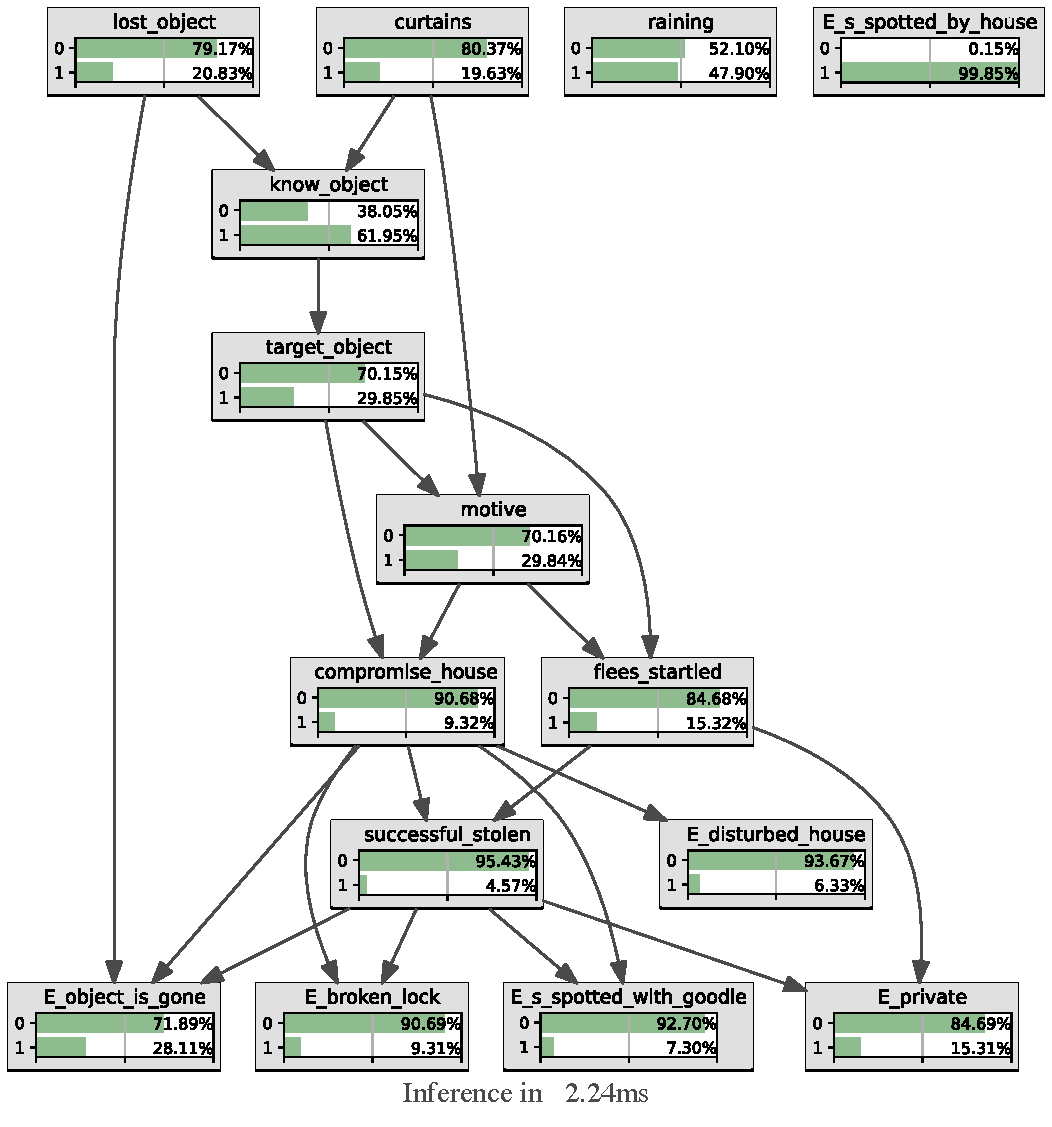
\includegraphics[width=\linewidth]{../experiments/StolenLaptopVision/bnImage/BNIMAGEStolenLaptopVision.pdf}
\caption{network structure}
\label{visionlaptopAcc}
\end{subfigure}
\end{center}

\begin{subfigure}{.5\textwidth}

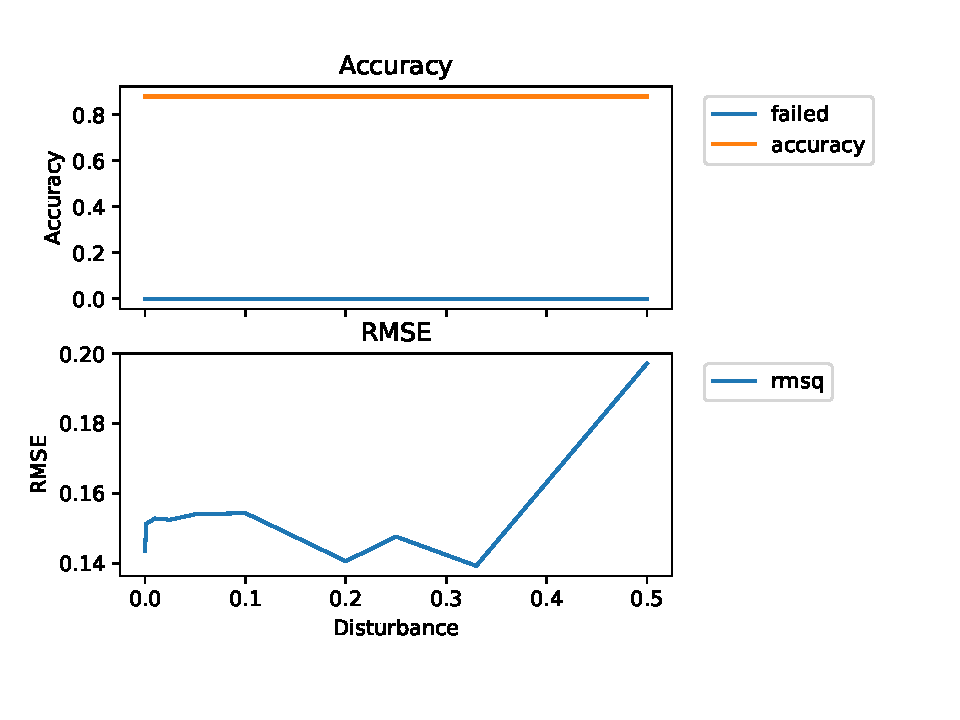
\includegraphics[width=\linewidth]{../experiments/StolenLaptop/plots/performance_StolenLaptop.pdf}
\caption{Accuracy (100\% to 0\%) and Root Mean Square error (1 - 0) }
\label{laptopAcc}
\end{subfigure}
\begin{subfigure}{.5\textwidth}
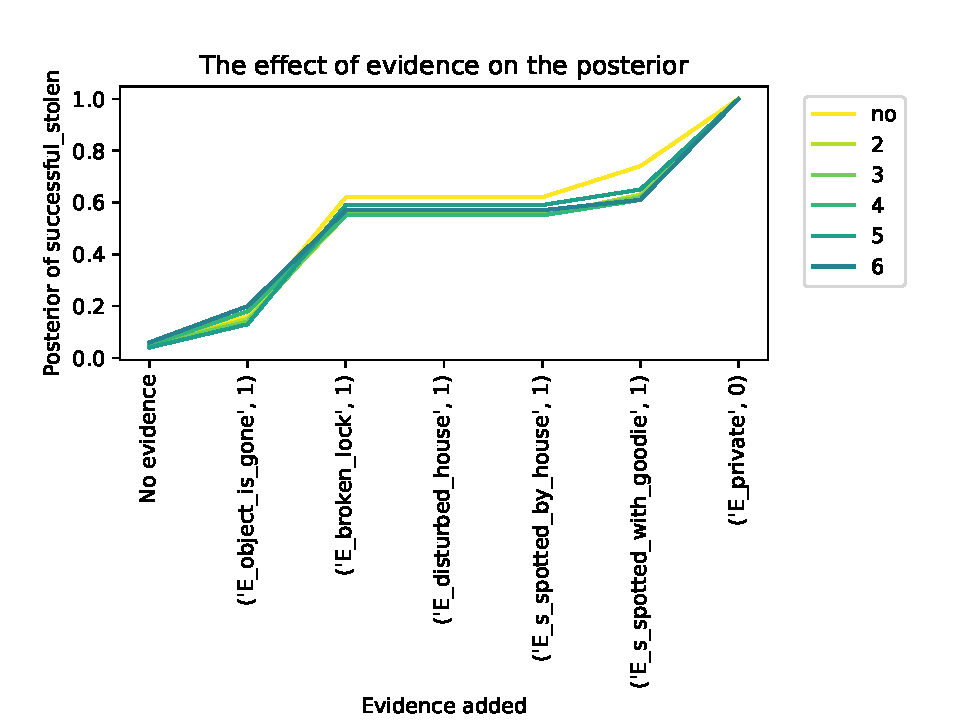
\includegraphics[width=\linewidth]{../experiments/StolenLaptopVision/plots/posterior_StolenLaptopVision.pdf}
\caption{effect of evidence on posterior}
\label{visionlaptopPosterior}
\end{subfigure}
\caption{The network, the accuracy and root mean square for rounding the cpts to intervals, and the effect of evidence on the posterior for stolen laptop simulation.}
\label{vision}
\end{figure}



\subsection{Discussion}
We see here, that the name of the variable is actually incorrect. It shouldn't be called "agent seen near house", because the reporter is not actually reporting that the agent is near the house - instead it is reporting whether the agent is within the vision of the camera. So properly it should be called "agent is seen in camera", or we can rewrite the reporter to measure whether the agent is actually near the house. 

But, this means that the BN is not responsive to the effect of relevance in the real world. 


\section{Experiment 3: Investigating Private Knowledge}

\subsection{Introduction}
The most obvious problem in crime is the distribution of knowledge. The criminal will (usually) know what he did, victims can testify, the police knows something else. Etc. So our ultimate goal is just to collect all the private knowledge of all the people involved, and paint a collective knowledge picture that (ideally) everyone can agree on, and then the judge can decide. Of course, it is not in the interest of everyone to freely share their private knowledge all the time. Police might not want to talk about the limitations of their evidence (or their ways of procuring it), witnesses and victims might not want to talk due to incrimination, guilt/shame or relations to the people involved, and suspects might not want to share their murder plans (obviously). So there's so much private knowledge, and our Bayesian Network assumes that we can just get into the heads of everyone and report on what we find there. So what if we cannot? What if we lose some information - like that of the suspect: that the suspect will flee if it thinks that it is being observed?

\subsection{Method}
Drop column Private knowledge and evidence for it, see the effect on the posterior. See the effect on the disturbances.


\subsection{Results}


See Figure~\ref{private}

\begin{figure}[h]
\begin{center}
\begin{subfigure}{.50\textwidth}
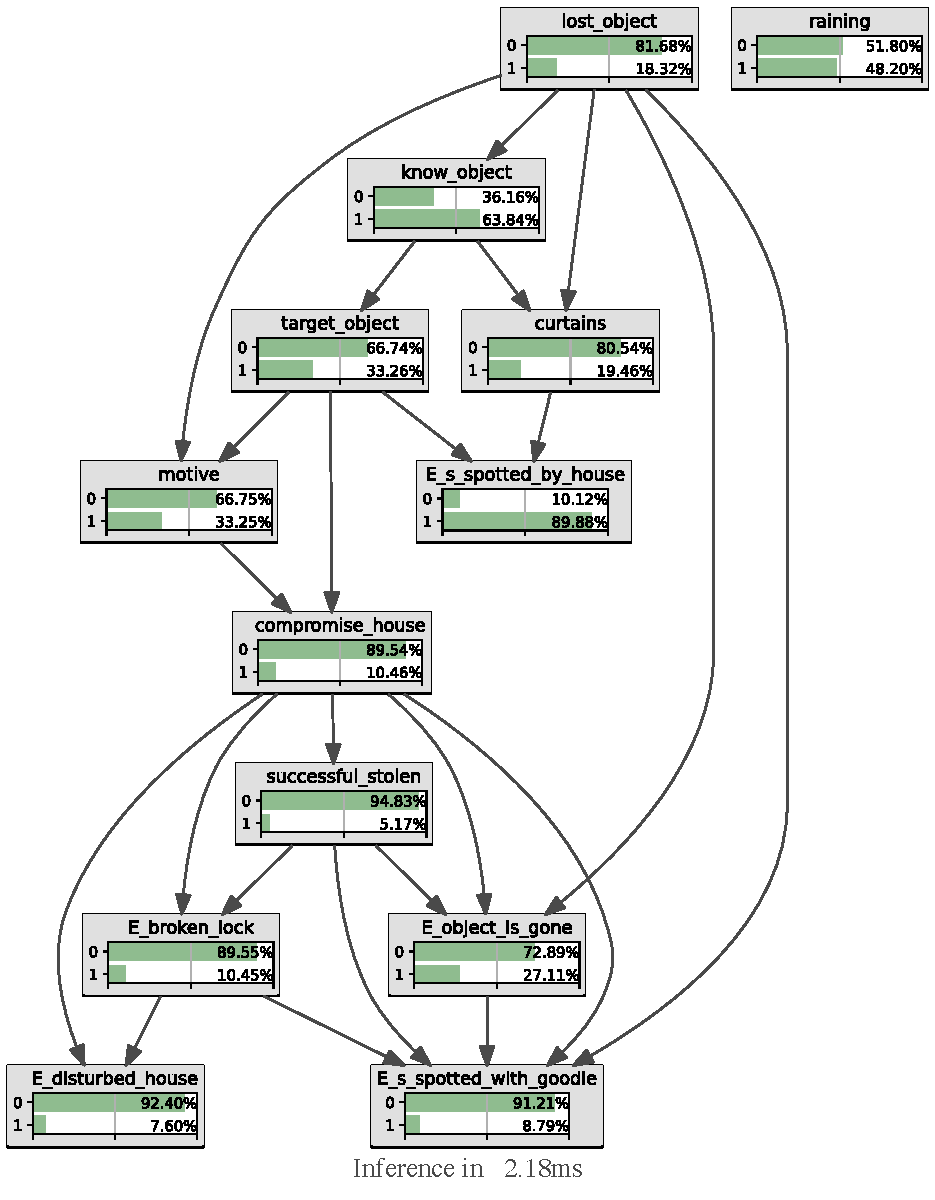
\includegraphics[width=\linewidth]{../experiments/StolenLaptopPrivate/bnImage/BNIMAGEStolenLaptopPrivate.pdf}
\caption{network structure}
\label{privatelaptopAcc}
\end{subfigure}
\end{center}

\begin{subfigure}{.45\textwidth}
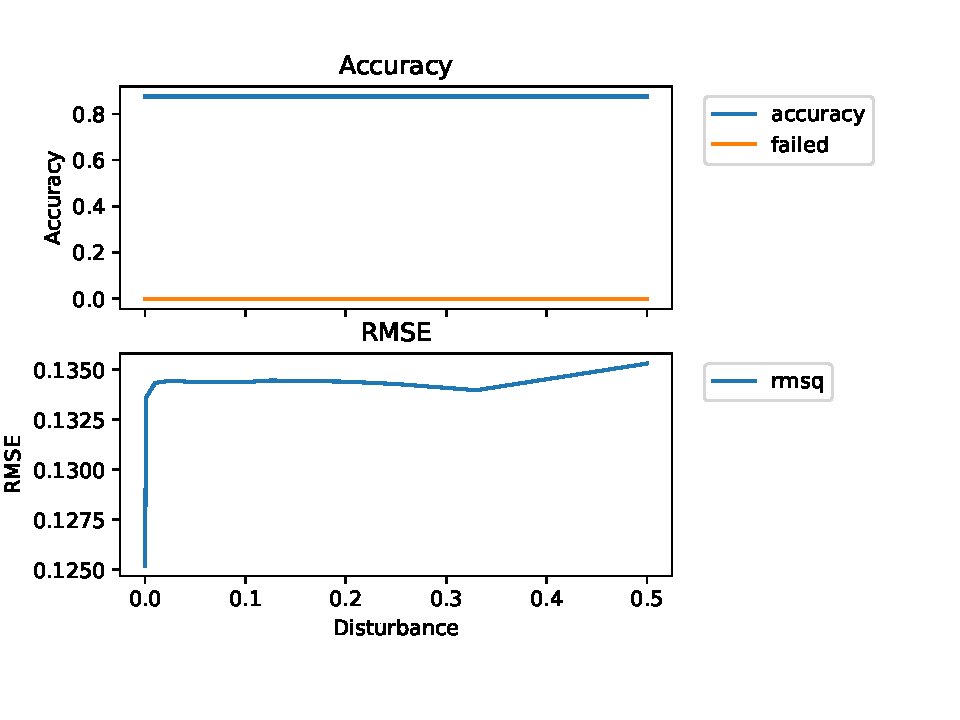
\includegraphics[width=\linewidth]{../experiments/StolenLaptopPrivate/plots/performance_StolenLaptopPrivate.pdf}
\caption{Accuracy (100\% to 0\%) and Root Mean Square error (1 - 0) }
\label{privatelaptopAcc}
\end{subfigure}

\begin{subfigure}{.45\textwidth}
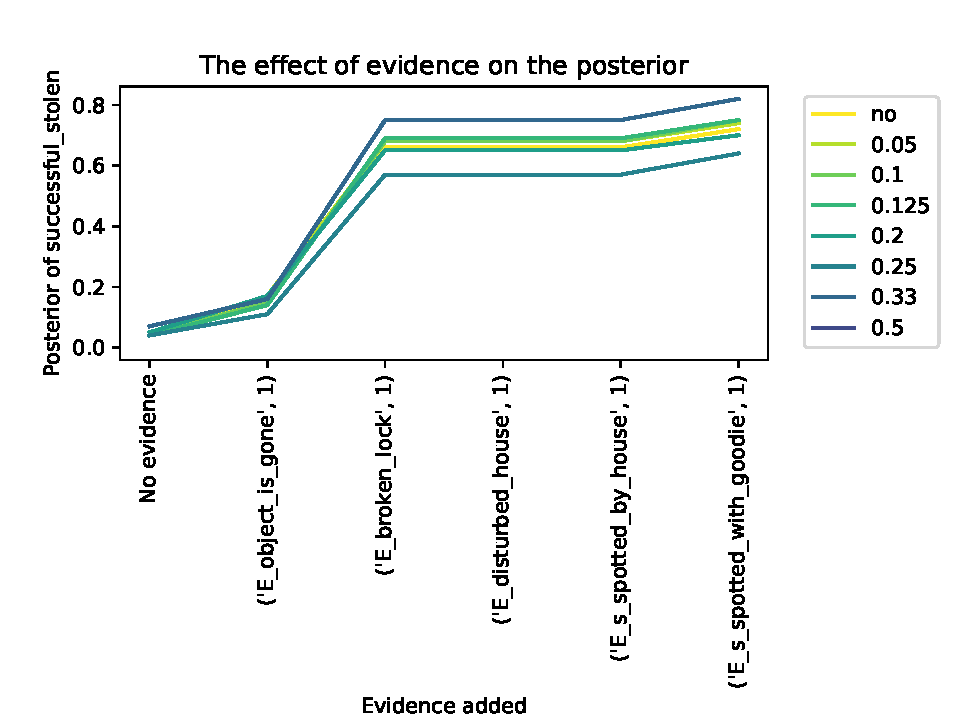
\includegraphics[width=\linewidth]{../experiments/StolenLaptopPrivate/plots/posterior_StolenLaptopPrivate.pdf}
\caption{posterior }
\label{privatelaptoppost}
\end{subfigure}

\caption{The network, the accuracy and root mean square for rounding the cpts to intervals, and the effect of evidence on the posterior for stolen laptop simulation.}
\label{private}

\end{figure}


\subsection{Discussion}

Seems to be effective, posterior never goes to 1. Lack of private knowledge hence will affect the end results, even if it will not affect the trajectory of the evidence progression. Overall accuracy and rms performs worse as well.


\section{Takeaways from the three experiments}



Simulating works, accuracy and RMS fine.

Table of accuracies and rms for the three experiments for comparisons.

We run into problems when we use words like `near' in our node names. We're lucky that we know what we mean (because our reporter forces us to make this explicit). We do not just ground the probabilities in our network, but we actually also ground our random variables - we have a measure of exactly what events we are interested in, and which we aren't.

We are in trouble with private knowledge, dropping this column from our table (which means that we don't know it) when we make our BN, we're drastically reducing our uh. Accuracy, and increasing our RMS. This implies that we do seem to need a full picture of everything that's happening, otherwise our BN will be kind of shit, and be less accurate :(.

Hence, for a simulation to work we 1) need to know exactly what it is that we're measuring since evidence strength depends on it \footnote{explain this more}, and 2) private information is necessary to create the BN because it influences fleeing behaviour. If we don't have this information our BN will be less effective.

\subsection{Forensic, Criminal and Legal interpreters, feasibility}
% how will a judge interpret this
If we assume that we can collectively build a network structure like the one that we have now, then there might be a lot of (good) room for legal interpretation. We have shown that this type of Bayesian Network does not have to be very precise. This leaves room for disagreements about probabilities: if we both made a subjective probabilistic estimation, because there's no good data available, and I think something is 20\% likely, and you think it's 30\% likely, we might still be able to agree on 25\%, and this would not result in a large decrease in accuracy of the network. As we've seen, accuracy only starts to decrease at thirds.

In these networks, we see that the evidence updates the posterior in the right direction - more evidence for stealing leads towards a higher value of `successful-stolen'. We also see the effects of different evidence strengths - knowing that the lock is broken is more important than seeing that the house is disturbed.

Forensic scientists will probably be annoyed by the lack of precision, but in these cases we do have a good operationalisation of what exactly is going on. Because we have this operationalisation, we can be sure that our data collection is correct. In the sci-fi world where police builds Bayesian Networks, I can imagine a situation where someone goes over all the files of all the crimes everyday, and collects statistics on occurances. However, the granularity of these crime files and the operationalisation are essential. Here, we can take them for granted. In real life, we cannot and that's a huge problem. 





			% 0
%\include{islandprior}				% 0!!!
% Activate the following line by filling in the right side. If for example the name of the root file is Main.tex, write
% "...root = Main.tex" if the chapter file is in the same directory, and "...root = ../Main.tex" if the chapter is in a subdirectory.
 
%!TEX root =  mainMastersProject.tex

\chapter[Conclusion]{Conclusion}

\section{Fundamental Problems with Bayesian Networks}

There are some fundamental problems with BNs as used for scenario-like whole legal Bayesian Networks.

Robustness is not the problem, even if we round to arbitrary intervals, losing a lot of precision, we have networks with a reasonable accuracy/rms error, that generally reach the right (enough) conclusion and respond correctly to evidence. Granularity is also whatever. The real problem is with the translation from human language to mathematical language. A random variable maps a sample world to a value, according to a certain procedure that is described in natural language. This means that for every node in the BN, we need to describe a procedure through which we can know whether or not it is true. This should be explicit, and everyone in court should agree with this - there can be no `personal interpretation' of this, no `probably close enough to count', because then we have shifted from one RV to a different one. This is not necessarily problematic, perhaps the robustness of BNs does not just hold for estimating a probability for a given reporter, but also holds for estimating a probability over an estimated set of reporters. However, we have to make this explicit - if we change reporters (RVs) without communicating about it, we're in trouble. 

However, in court this would imply that we would have a discussion about every measuring procedure for every node of every BN, and there would be no `idiom database', because as soom as we try to app
\subsection{Reporters, Reference Classes and Random Variables.}

Fundamentally, the problem is that the nodes in Bayesian Networks have a specific meaning. They are not pragmatic/dialogical/argumentation sentences, but have intricate statistical meaning \footnote{secret fourth good sherlock episode.} They are random variables, and a random variable implies an observation procedure (a mapping from a world state to a number). This means, that a node implies that we know how to measure if it is true or not in the real world.

 In our simulation, this is really not a problem. We have an observation procedure: if a certain state occurs, we have the reporter in the same place as when the state change occurs, and the reporter reports exactly and only that. In experiment XXX we saw what happens when this goes wrong: if we have an imprecise/contradictory/smaller/larger reporters, we see that the probabilities can change a lot, might even change the structure of the network. 
 
Hence, BNs might work for subsections of reality that have a clear observation procedure (eg reasoning with DNA evidence or other forensic stuff). We know exactly what it means for the node to be true (eg: we know the measurement associated with the random variable). However, for many of the node events that we encounter in scenario BNs/argumentation BNs, we do not know how we are determining that the node is true or not. So either we spell out exactly when a node is true or not, and by exactly I mean exactly, and we lose all generality/chance at DBs. Or we do not spell it out, interpret BN nodes not as random variables but as some sort of fuzzy conditional logic operation, but then that's fine, but we're not really building Bayesian Networks, we're doing something else.

Experiment outcomes: best possible case would be that the structure of the BN becomes different (not just the probabilities) based on different reporters used.

- I want one random variable that is a `wide' interpretation: a combination of all possible reporters for some thing.
- I want some random variables that are the most narrow possible interpretation.
- alternative.

---------------------------------------------------------------------

This is not the same as the problem of the reference class, but it is related. The problem of the reference class is the discussion which definition/reporter is appropriate for a given situation. This problem is the step before that, which is - how do we specify what reference class we are talking about? This is not described in the scenario-like BNs I've discussed in my introduction. The forensic BNs come closer, because there we at least know what method is used to determine if an event happened or not...

\subsection{Maps and implicitness.}

Put the exact same agents with the same behavioural loops on a different map, and the probabilities for events change (see XXX). This is not a problem - this means that environment/world knowledge/context, which is not a node explicitly in the Bayesian Network, affects the output of networks. This can be remedied in a sense, by adding a context node. So what's the problem? That if we see a BN and we do not know exactly what the context was in which it was created, we cannot assume that it generalises to a different environment. We cannot take parts of that network (with probabilities) and put it in a different one, because implicitly it is only defined over the environment for which it was originally created.

\subsection{Private knowledge}

Here we run into a paradox: in our simulation we know exactly when something is true, even when that thing is private knowledge. If we leave out the private knowledge (drop from our table, basically), we have a problem and the accuracy of the network drops. This means that we can only generate a BN that uses private knowledge if we have all knowledge, requiring everyone in the process to help along. Feasible? No.


\section{Conclusion}
Bayesian Networks are a good tool if you know exactly what you want to investigate and have methods for it as well. This is the case in simulation, obviously.


\section{Future Work}
Testing or generating Bayesian Network idioms from simulations. The dream is to get ``plug and play'' Bayesian Network idioms - preconnected structures (perhaps even with some probabilities attached) that you can add evidence to and adapt and combine if necessary. Using simulations, we can test the granularity of these possible idioms, to simulate a crime at larger and smaller resolution (more or fewer events) to see how well the idioms can capture it.

Investigate the effect of granularity, expecially in relation to the complexity of the network. Size, num of arrows, etc. 				% 0







\bibliographystyle{plain-annote}
\bibliography{mybibliography}


\end{document}
\end

